\chapter{Modellbeschreibung}\label{Modellbeschreibung}
\section{Erzeuger}\label{Erzeuger}

Im folgenden wird gezeigt, auf welcher Grundlage die Erzeugungsanlagen in den jeweiligen Inselnetzen modelliert werden. In Anlehnung an den Abschlussbericht des Umweltbundesamtes zur Transformation der Stromerzeugung bis 2050 wird der Fokus ausschließlich auf die Modellierung von Windenergie- und Photovoltaikanlagen gelegt, da diese den Großteil der Erzeugung in allen betrachteten Szenarien darstellen. Zudem bieten sich diese Erzeugungsanlagen besonders für den autarken Einsatz in Inselnetzen an.

\subsection{Wetterdaten}

Die verwendeten Erzeugungsanlagen setzen eine Simulation von Wetterdaten voraus. Für Windenergieanlagen ist daher die Windgeschwindigkeit in $m/s$  und für die Photovoltaikanlagen die Summe der Globalstrahlung der vorangegangenen 10 Minuten in $J/cm^2$ von Bedeutung. Diese Daten stellt der deutsche Wetterdienst für über 400 verschiedene Wetterstationen in Deutschland im csv-Dateiformat frei zur Verfügung. Zudem werden die Daten in einer 10-minütigen Auflösung gemessen und bereitgestellt. Für die folgenden Simulationen werden Wetterdaten der anschließend aufgeführten Wetterstionen verwendet.

\begin{center}
	\begin{tabular}[htpb]{c|c|c|c|c}
		Stations ID & Stationshöhe & Länge & Breite & Standort \\
		\hline
		00691 & $4~m$ & 53.0451 & 8.7981 & Bremen \\
		02115 & $4~m$ & 54.1860 & 7.9119 & Helgoland \\
		00282 & $240~m$ & 49.8743 & 10.9206 & Bamberg 
	\end{tabular}
\end{center}

Die Verläufe der Windgeschwindigkeit und Globalstrahlung der beiden Wetterstationen für die Jahre 2020 bis 2022 sind in \autoref{fig:wetter} zu sehen.

\begin{figure}[H]
	\centering
	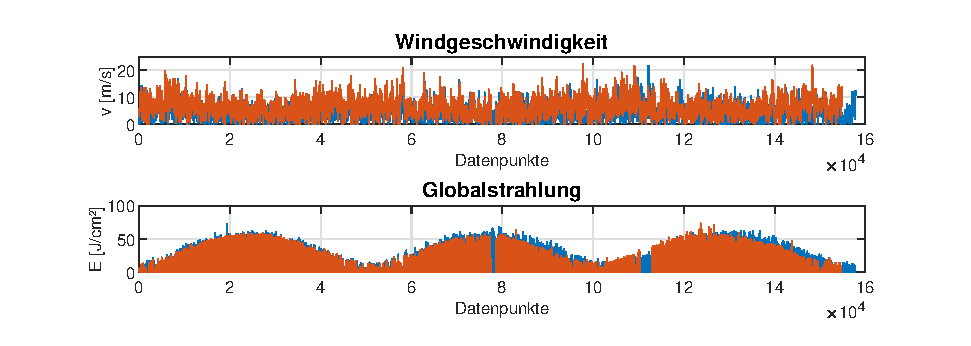
\includegraphics[width=\linewidth]{Abbildungen/Wetter20bis22.eps}
	\caption{Wetterdaten für die Standorte Bremen Flughafen und Helgoland für die Jahre 2020 bis 2022}
	\label{fig:wetter}
\end{figure}

Die Wetterstation in Bremen befindet sich auf freier Fläche in der nähe des Bremer Flughafens und spiegelt daher die Wetterverhältnisse im Umkreis von Bremen wieder. Zur Simulation einer Insel dient die Wetterstation auf Helgoland. Wie in \autoref{fig:wetter} zu erkennen, zeichnet sich hier das Wetter vor allem durch die höhere Windauslastung aus. Die Globalstrahlung ist größtenteils identisch.

\subsection{Windenergie}

Um das Erzeugungsverhalten einer Windenergieanlage zu beschreiben wird im wesentlichen der Zusammenhang zwischen der Windgeschwindigkeit und der ausgegebenen elektrischen Leistung der Anlage benötigt. Als Ansatz hierfür dient die kinetische Energie $E_{kin}$ einer Luftmasse $m$ mit der Geschwindigkeit $v$. \cite{Hau2016}

\begin{equation}
	E_{kin} = \frac{1}{2} mv^3
	\label{eq:wind}
\end{equation}

Im Falle eines Rotors wird eine bestimmte Querschnitsfläche $A$ betrachtet, durch die ein Massenstrom $\dot{m}$ strömt. Dieser lässt sich mithilfe der Luftdichte $\rho$ nach \cite{} wie folgt ausdrücken:

\begin{equation}
	\dot{m} = \rho vA
\end{equation}

Mit Einsetzen in \autoref{eq:wind} ergibt sich somit die enthaltene Leistung im Wind, da die Masse durch den Massenstrom ersetzt wird und sich somit die Energie pro Zeit (Leistung) ergibt.

\begin{equation}
	P_{Wind} = \frac{1}{2}\rho A \nu^3
\end{equation}

%\begin{figure}[H]
%	\centering
%	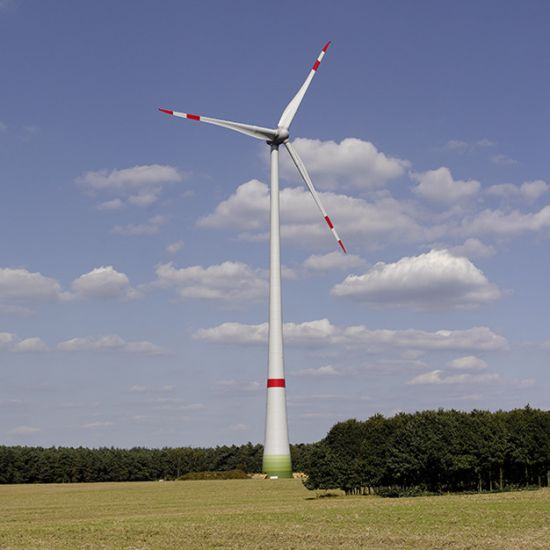
\includegraphics[width=0.7\linewidth]{Abbildungen/E115.jpg}
%	\caption{Enercon E-115}
%	\label{fig:e115}
%\end{figure}
Es zeigt sich, dass die Leistung kubisch von der Windgeschwindigkeit abhängt. Die im Wind enthaltene Leistung wird jedoch nicht vollständig in einer Windenergieanlage in elektrische Leistung umgesetzt. Den Zusammenhang zwischen der Windgeschwindigkeit und der erzeugten Leistung stellt die Leistungskurve einer Anlage dar. Beispielhaft zeigt \autoref{fig:Leistungskurve} die Leistungskurve einer Windenergienalage der Herstellers Enercon. 

\begin{figure}[H]
	\centering
	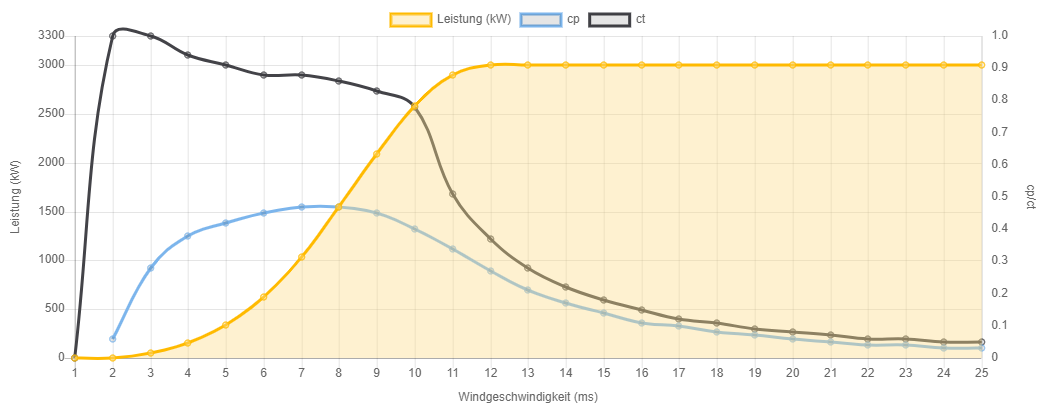
\includegraphics[width=0.9\linewidth]{Abbildungen/Enercon E115.png}
	\caption{Leistungskurve Enercon E-115 \cite{E115}}
	\label{fig:Leistungskurve}
\end{figure}

Dieser Anlagentyp und die zugehörige Leistungskurve dienen auch für die weiteren Simulationen als Datengrundlage. Weitere Parameter, welche für die Simulation relevant sind, werden im folgenden veranschaulicht.

\begin{center}
	\begin{tabular}[htpb]{c|c}
		Typ & Enercon E-115 \\
		\hline
		Nabenhöhe & $149~m$ \\
		Einschaltgeschwindigkeit & $2~m/s$ \\
		Abschaltgeschwindigkeit & $25~m/s$
	\end{tabular}
\end{center}

Wie \autoref{eq:wind} zeigt, ist die erzeugt Leistung stark von der Windgeschwindigkeit abhängig. Diese nimmt wiederum mit steigender Höhe tendenziell zu, weshalb eine Betrachtung der Windgeschwindigkeit in Nabenhöhe notwendig ist. Da die Wetterdaten jedoch meistens in deutlich geringeren Höhen gemessen werden, wird zur Schätzung der Windgeschwindigkeit das logarithmische Windprofil verwendet. Mithilfe von \autoref{eq:log} lässt sich mit der gemessenen Widngeschwindigkeit in einer Höhe unter Angabe der Rauigkeit der Umgebung die Windgeschwindigkeit in einer gewünschten Höhe abschätzen. \cite{Hoehenprofil}

\begin{equation}
	v(h) = \frac{v_{Ref}}{ln\left(\frac{h_{Ref}}{z_0}\right)} \cdot ln\left(\frac{h}{z_0}\right)
	\label{eq:log}
\end{equation}

Mit:

\begin{flushleft}
	\begin{tabular}[htpb]{ll}
		$v(h)$: & Windgeschwindigkeit in Höhe $h$ \\
		$h$: & Höhe über dem Boden \\
		$z_0$: & Bodenrauigkeit \\
		$v_{Ref}$: & Windgeschwindigkeit in Referenzhöhe $h_{Ref}$ 
	\end{tabular}
\end{flushleft}

Bei der Messung in Bodennahen Schichten spielt vorallem die Bodenrauhigkeit eine maßgebliche Rolle, da die Messung hier von der Umgebung stark beeinflußt wird. \autoref{tab:Rauigkeit} zeigt daher die anzunehmenden Werte, je nach Standort der Messstation.  

\begin{table}[H]
	\begin{tabular}[htpb]{p{4cm}|p{3cm}|p{7cm}}
		\textbf{Rauhigkeitsklasse} & \textbf{Rauhigkeitslänge} & \textbf{Geländetyp} \\
		\hline
		0 & 0,0002 & Wasserflächen \\
		\hline
		0,5 & 0,0024 & Offenes Terrain mit glatter Oberfläche, z. B. Beton, Landebahnen auf Flughäfen, gemähtes Gras \\
		\hline
		1 & 0,03 & Offenes landwirtschaftliches Gelände ohne Zäune und Hecken, eventuell mit weitläufig verstreuten Häusern, sehr sanfte Hügel \\
		\hline
		1,5 & 0,055 & Landwirtschaftliches Gelände mit einigen Häusern und 8 Meter hohen Hecken im Abstand von ca. 1.250 Meter \\
		\hline
		2 & 0,1 & Landwirtschaftliches Gelände mit einigen Häusern und 8 Meter hohen Hecken im Abstand von ca. 500 Meter \\
		\hline
		2,5 & 0,2 & Landwirtschaftliches Gelände mit vielen Häusern, Büschen, Pflanzen oder 8 Meter hohen Hecken im Abstand von ca. 250 Meter \\
		\hline
		3 & 0,4 & Dörfer, Kleinstädte, landwirtschaftliche Gebäude mit vielen oder hohen Hecken, Wäldern und sehr raues und unebenes Terrain \\
		\hline
		3,5 & 0,8 & Größere Städte mit hohen Gebäuden \\
		\hline
		4 & 1,6 & Großstädte, hohe Gebäude, Wolkenkratzer \\
	\end{tabular}
\centering
\caption{Angenommene Parameter für die Validierung der Berechnungsmethode \cite{Rauigkeit}}
\label{tab:Rauigkeit}
\end{table}

Von der Tabelle ausgehend wird für den Standort Bremen Flughafen eine Rauhigkeitsklasse von 0,5 angenommen, da sich die Wetterstation direkt neben einer Landebahn befindet. Für die Messung auf Helgoland wird hingegen eine Rauhigkeitsklasse von 1 angenommen, aufgrund der geringen Höhe der Messtation in Kombination mit einer leicht hügeligen Umgebung.

Die zuvor beschriebenen Zusammenhänge werden nun in einem Simulink Modell verknüpft. Es ergibt sich das Modell in \autoref{fig:simulinkWEA}.

\begin{figure}[H]
	\centering
	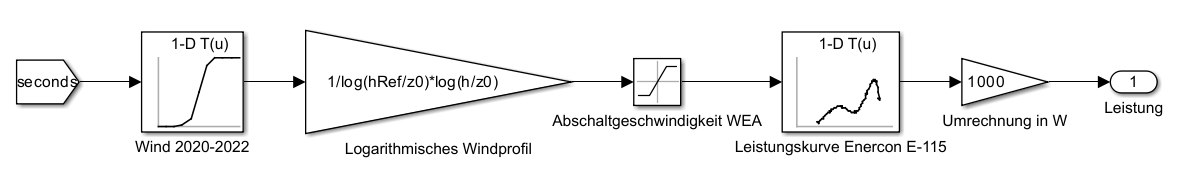
\includegraphics[width=0.9\linewidth]{Abbildungen/ModellWEAeinfach.png}
	\caption{Simulink Modell einer Enercon E-115}
	\label{fig:simulinkWEA}
\end{figure}

Zur Betrachtung des Modells in einem dreiphasigen Netz wird das Modell um einen Dreiphasigen Erzeugerblock ergänzt. Auf eine detaillierte Betrachtung des elektrischen und mechanischen teils der Windenergieanlage wird verzichtet, da dieser für die oberflächliche Betrachtung im Rahmen dieses Projekts keine Rolle spielt. Zudem erhält das Modell zwei PT1-Glieder um die Trägheit der Erzeugung darzustellen. Die Verbindung der Phasen zum Netz über einen Widerstand dient zur Stabilität des Modells während der Simulation.

\begin{figure}[H]
	\centering
	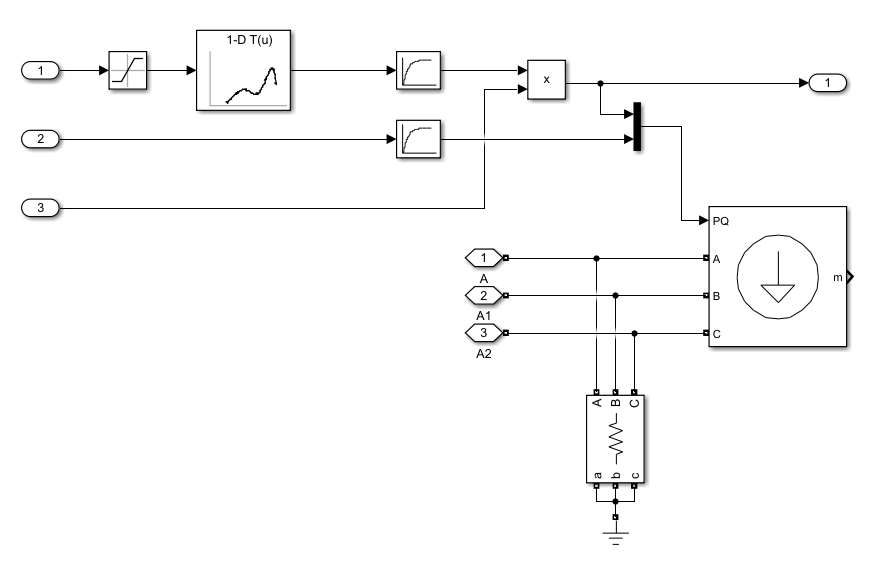
\includegraphics[width=0.9\linewidth]{Abbildungen/ModellWEA.png}
	\caption{Simulink Modell einer Enercon E-115}
	\label{fig:e115}
\end{figure}

\subsection{Photovoltaik}

Ähnlich wie bei der Windenergieanlage wird zur Modellierung einer Photovoltaikanlage ein Bezug zwischen der in der Sonnenstrahlung enthaltenen Energie und der ausgegebenen elektrischen Energie eines PV Moduls hergestellt. Nach \cite{PV} besteht ein proportionaler Zusammenhang zwischen der elektrischen Leistung eines PV-Moduls $P_{el}$ und dem Strahlungsfluss $\Phi$. 

\begin{equation}
	P_{el} = \eta \cdot \Phi
\end{equation}

Der Strahlunfsluss $\Phi$ berechnet sich aus der Starhlungsdichte $E$ und der Fläche $A$. Bei homogener Bestrahlung ergibt sich der folgende Zusammenhang.

\begin{equation}
	\Phi = E \cdot A
\end{equation}

Die Strahlungsdichte $E$ entspricht der gemesenenen Globalstrahlung der betrachteten Wettestaiuonen.

Die Leistung des Strahlungsflusses wird dabei mit dem Modulwirkungsgrad $\eta$ in elektrische Leistung umgewandelt. Die Verluste sind in \autoref{fig:VerlustePV} in einem Sankey-Diagramm Veranschaulicht. 

\begin{figure}[H]
	\centering
	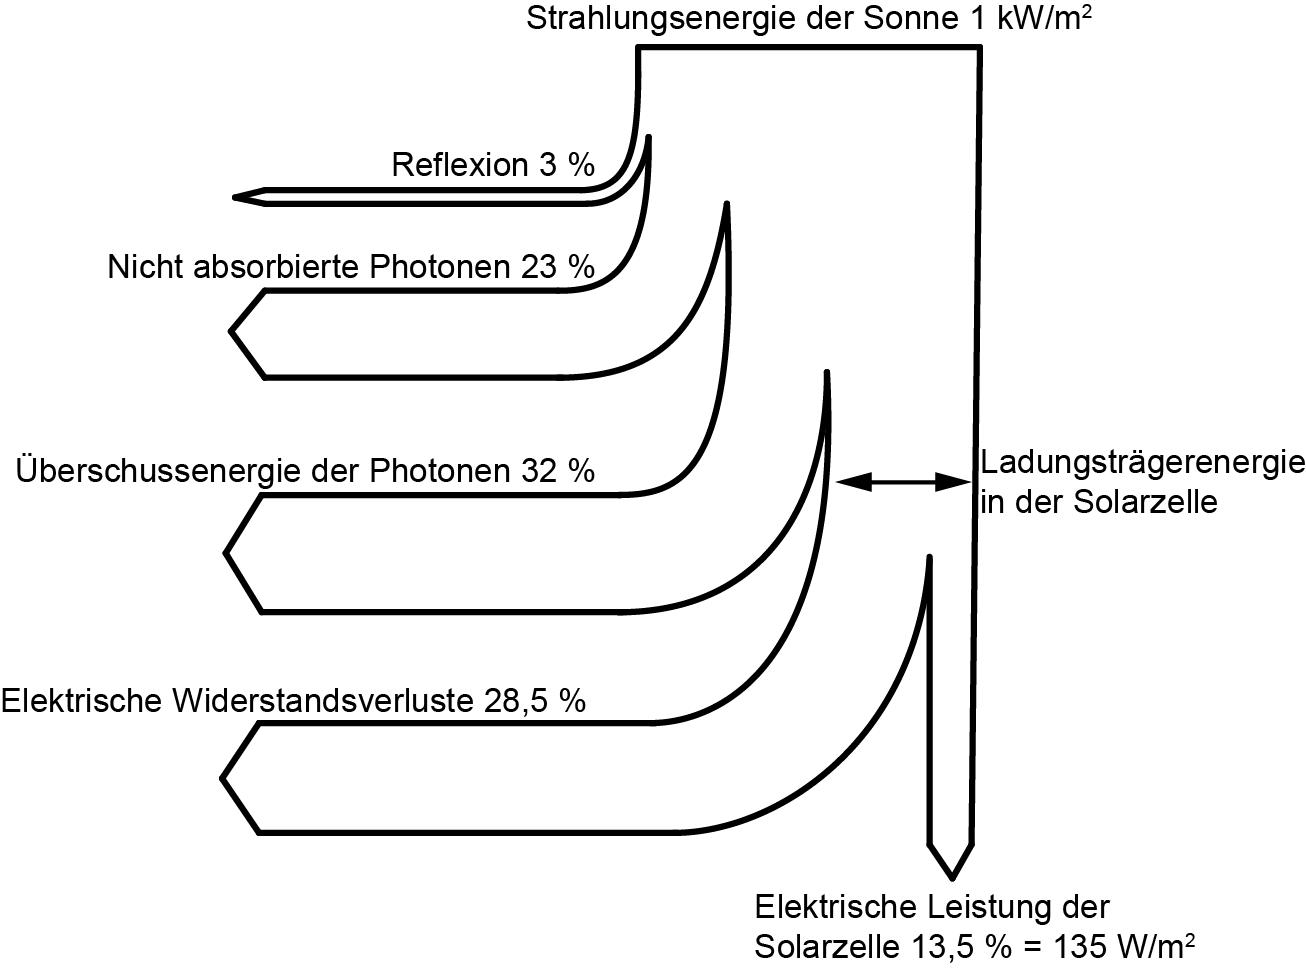
\includegraphics[width=0.7\linewidth]{Abbildungen/WirkungsgradPV.png}
	\caption{Veranschaulichung der Verluste innerhalb eines PV-Moduls mithilfe eines Sankey-Diagramms \cite{VerlustePV}}
	\label{fig:VerlustePV}
\end{figure}

Der hier angegebene Modulwirkungsgrad ist jedoch etwas veraltete und die Wirkungsgrade von Solarmodulen steigen kontinuierlich um etwa 0,3 - 0,5 \%-Punkte pro Jahr, sodass sich aktuell ein Wikrungsgrad von ungefähr 21~\% für kommerzielle Solarmodule ergibt. Im Betrieb wirken sich noch diverse andere nichtlineare Effekte auf den Modulwirkungsgrad aus wie z.B. die Modultemperatur, Verschattung oder die Verschmutzung der Module. Zudem ergeben sich noch zusätzliche Verluste in den Leitungen, Wechselrichtern und Transformatoren der Photovoltaikanlage. Die hier ntstehenden Verluste sind jedoch eher Vernachlässigbar, da beispielsweise Wechselrichter üblicherweise einen Wirkungsrad von 98~\% erreichen. Mit Betrachtung der sonstigen Einflusse auf den Wirkunsgrad wird ein mittlerer Wikrungsgrad von 18~\% zwischen der Strahlungsdichte und der elektrischen Leistung der Anlage angenommen. \cite{FaktenPV} 

Werden die beschriebenen Zusammenhänge in ein Simulink-Modell transferiert, ergibt sich das Modell in \autoref{fig:PVModell}

\begin{figure}[H]
	\centering
	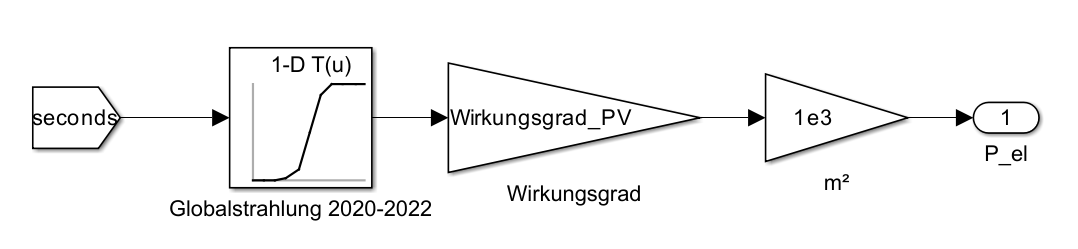
\includegraphics[width=0.9\linewidth]{Abbildungen/PVModell.png}
	\caption{Starkl vereinfachtes Modell einer PV-Anlage in Simulink}
	\label{fig:PVModell}
\end{figure}

Dabei handelt es sich um ein stark vereinfachtes Modell, welches jedoch für diese Betrachtung völlig ausreichend ist, da es die Fluktuation der Sonnenstrahlung wiedergibt und diese für die Bestimmung der Leistungsbilanz ausschlaggebend ist.

\section{Verbraucher}

Wie in \autoref{ch:Theorie} dargestellt, erfolgt die Simulation der Verbraucher auf Grundlage von Lastprofilen. Diese werden, wie in \autoref{fig:Last} zu sehen, mithilfe von zweidimensionalen Look-Up-Tables in das Modell integriert. 

\begin{figure}[H]
	\centering
	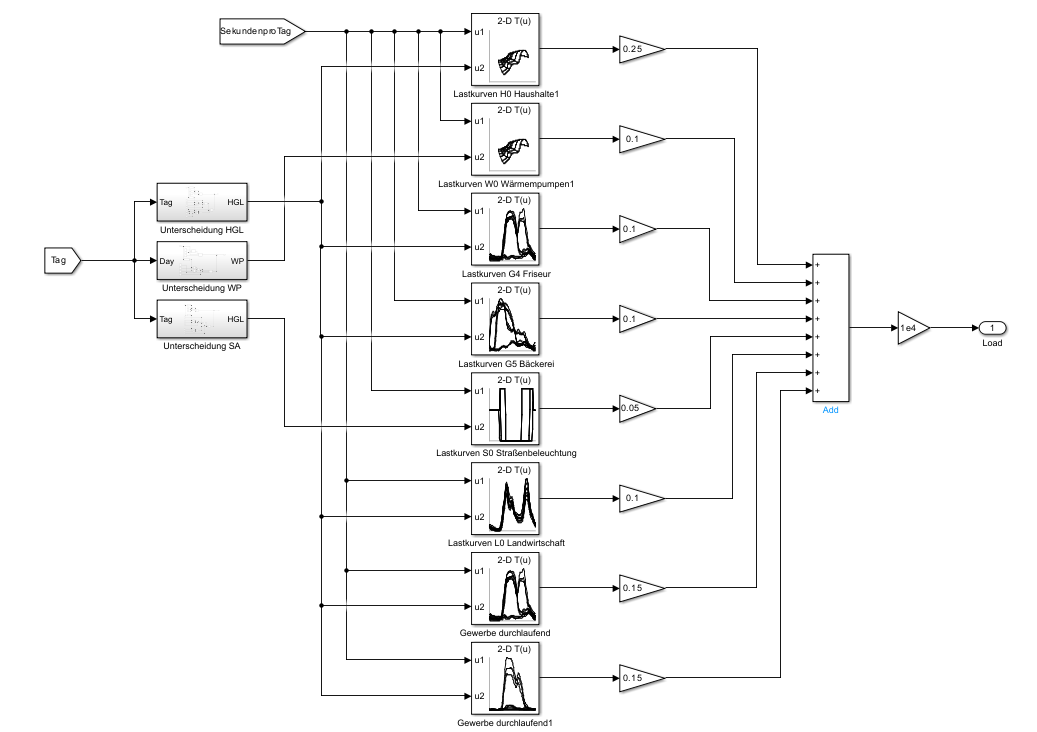
\includegraphics[width=0.9\linewidth]{Abbildungen/LastBilanziell.png}
	\caption{Simulink Modell zur Simulation einer beliebigen Stromlast}
	\label{fig:Last}
\end{figure}

Die Lastverläufe sind jeweils von der Uhrzeit, dem Wochentag und der Jahreszeit abhängig. Daher wird zu beginn mithilfe einer logischen Schaltung zwischen den jeweiligen Wochentagen und Jahreszeiten unterschieden. Anschließend wird anhand des Zeitpunktes ein Lastwert für jedes Standardprofil bestimmt. Die verschiedenen Lastprofile fließen durch einen Gewichtungsfaktor in unterschiedlichen Anteilen in die Berechnung der Gesamtlast ein. Zuletzt wird noch ein Skalierungsfaktor benutzt, um die Last auf eine gewünschten Jahresverbrauch anzupassen. Da alle Lastprofile auf einen Jahresverbrauch von 1000~kWh/a normiert sind, gibt dieser Faktor den Gesamtjahresverbrauch in vielfachen von 1000~kWh/a an.
\section{Speicher}\label{Speicher}
In diesem Abschnitt soll der Aufbau und die Steuerung der Speichermodelle erläutert werden.
Dazu werden zunächst verschiedene Batteriemodelle eingeführt und anschließend der gewählte Aufbau für
unsere Simulationen gezeigt. 
Zusätzlich soll die Umsetzung der in Abschnitt~\ref{Betriebsstrategien} angeführten Betriebsstrategien 
beschrieben werden.

\subsection{Batteriemodelle}\label{Batteriemodelle}
Batteriemodelle können grundlegend in 
%\begin{itemize}
%    \item mathematisch, empirische Black-Box-Modelle,
%    \item elektrische Modelle und
%   \item physikalisch-chemische Modelle
%\end{itemize}
unterteilt werden. 
Innerhalb dieser Kategorien gibt es zusätzlich erhebliche Unterschiede in Bezug auf die Komplexität des Modells.
Die mathematischen Modelle versuchen dabei, das Verhalten von Batterien durch Umsetzung von empirisch bestimmten
Zusammenhängen abzubilden.
So können aus festgelegten Kennparamatern in Verbindung mit Eingangsgrößen die jeweiligen Ausgangsgrößen berechnet werden.
Dabei unterscheiden sich die verschiedenen Modellvarianten stark in ihrer Betrachtung einzelner Aspekte.

In der Kategorie der elektrischen Batteriemodelle wird versucht das Verhalten von Batterien durch Ersatzschaltkreise
mit einfachen elektrischen Bauteilen nachzubilden.
Auch hierbei gibt es große Unterschiede im detailgrad der einzelnen Umsetzungen, es besteht aber die Möglichkeit
auch komplexe elektrochemische Effekte zu modellieren.

Zuletzt bilden die physikalisch-chemischen Modelle wohl die aufwändigste Form.
Durch sie wird versucht auch das Zusammenspiel der einzelnen Materialien innerhalb der Batterie nachzubilden.
Dadurch kann das Verhalten einzelner Batteriezellen sehr genau untersucht werden, in der Praxis sind diese
Modelle aber eher selten zu finden, da die Zusammenhänge auf einer so detaillierten Ebene nur schwer zu ermitteln sind
und Simulationen eher auf das Gesamtverhalten von Batteriesystemen abzielen~\parencite[]{keil2012aufbau}.

Für unsere Simulationen haben wir uns für ein mathematisches Black-Box-Modell entschieden, dass es uns ermöglicht
die Spannung, Leistung und den SOC des Batteriemodells zu betrachten.
Auf Grund der vereinfachten Umsetzung und der insgesamt trotzdem hohen Komplexität des gesamten Simulationsmodells
sollte so die Simulationsdauer möglichst gering gehalten werden.

\begin{figure}[h!]
    \centering
    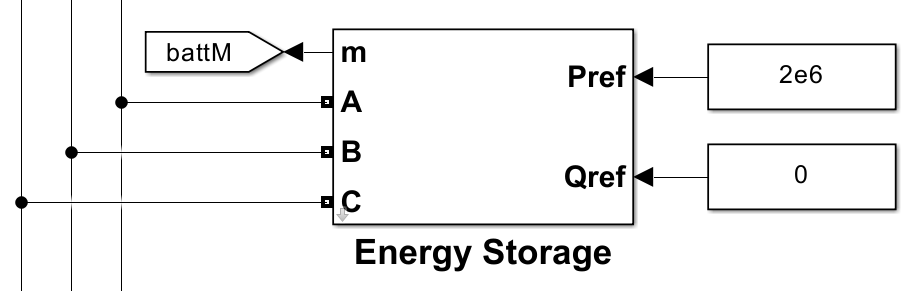
\includegraphics[width=8cm]{Abbildungen/BatterieBlackBox.png}
    \caption{Subsystem-Baustein der Batterie in Simulink}\label{BatModell}
\end{figure}
Abbildung \ref{BatModell} zeigt den Batterie-Block mit den Eingängen zur Wirk- und Blindleistung und den 
Ausgängen für jede Spannungsphase sowie dem Ausgang der Messgrößen.

\begin{figure}[h!]
    \centering
    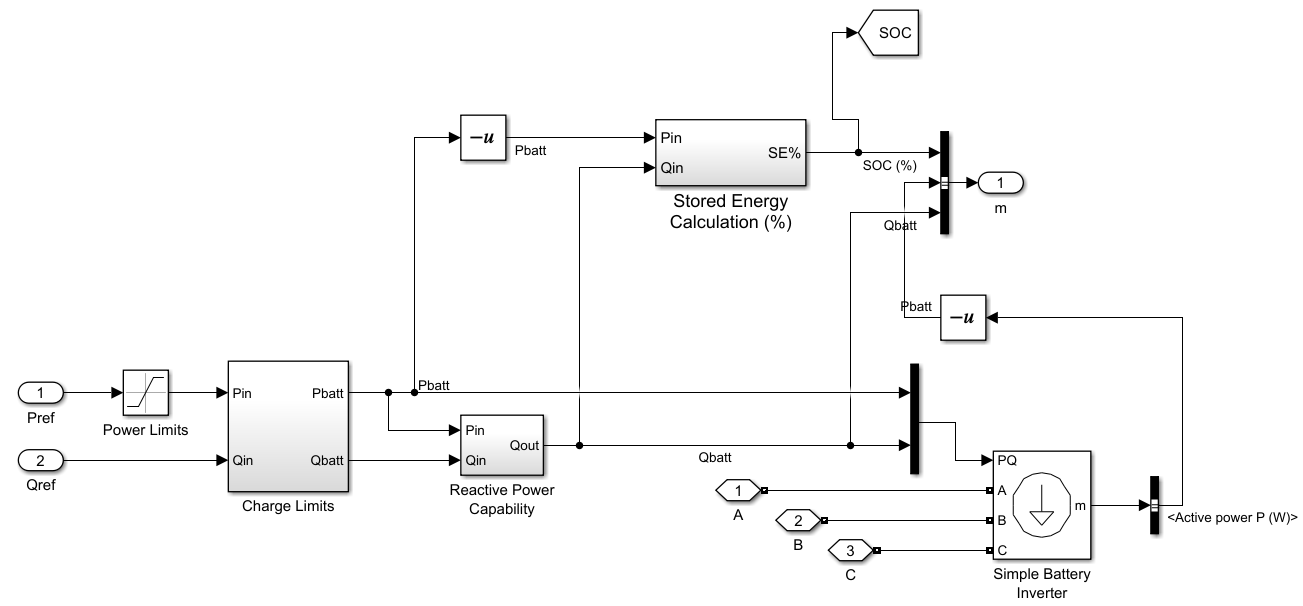
\includegraphics[width=14cm]{Abbildungen/Speicher Ebene1.png}
    \caption{Inhalt des Batteriesubsystems in Simulink}\label{BatModell1}
\end{figure}

Der Aufbau des Subsystems ist in Abbildung~\ref{BatModell1} gezeigt.
Im Wesentlichen besteht das Modell aus einem Block zur Steuerung und Umsetzung der Betriebsstrategien, einem Block
zur Berechnung des SOCs und einer dreiphasigen Last die für dieses Modell als einfacher Umrichter genutzt wird.
Thermische Effekte, Verzögerungen oder Nicht-Linearitäten wurden beim Entwurf dieses Modells gänzlich vernachlässigt.
Auch Selbstentladungseffekte oder Aussagen über die Lebensdauer des Batteriespeichers können mit diesem Modell nicht 
betrachtet werden.

Zur Auswertung der Betriebsstrategien und zum groben Entwurf eines realistischen Inselnetzes sollte die Komplexität
des Modells dennoch genügen.
Trotz dieser starken Vereinfachungen laufen Simulationen im dreiphasigen Modell fast in Echtzeit ab.

Während die Steuerung im nächsten Abschnitt~\ref{Lade- und Entlade} genauer erläutert wird soll hier auf die anderen
Komponenten des Batteriemodells etwas näher eingegangen werden.

\paragraph{SOC-Schätzung}
Der Block zur SOC-Schätzung (im Modell als Stored Energy Calculation bezeichnet) basiert auf einem einfachen Leistungsintegral.
Dabei wird aus dem Integral der Batterieleistung die gespeicherte Energiemenge berechnet, welche dann mit der Kapazität der Batterie verglichen wird.
Der SOC zum Zeitpunkt t ergibt sich dann aus
\begin{equation}\label{GL_SOC}
	SOC_{\%}(t) = \frac{E(t)}{C} \cdot 100
\end{equation}
mit
\begin{equation}\label{GL_SOC2}
	E(t) = \int_{0}^{t}p(t) \diff t + E(0) = \int_{0}^{t}p(t) \diff t + \frac{SOC_{\%}(0)}{100}\cdot C.
\end{equation}
Wobei hierbei die korrekte Form der Einheiten zu beachten ist.
Ist die Kapazität der Batterie in $kWh$ gegeben muss das Integral der Leistung entsprechend umgerechnet werden.
Des Weiteren muss der Momentanwert der Leistung zunächst aus Blind- und Wirkleistung bestimmt werden.
Abbildung~\ref{SOC} zeigt die Umsetzung der beiden Gleichungen~\ref{GL_SOC} und~\ref{GL_SOC2} im Simulink-Modell 
wobei der anfängliche Ladezustand im Integral-Block als Anfangszustand hinterlegt ist.
\begin{figure}[h!]
	\centering
	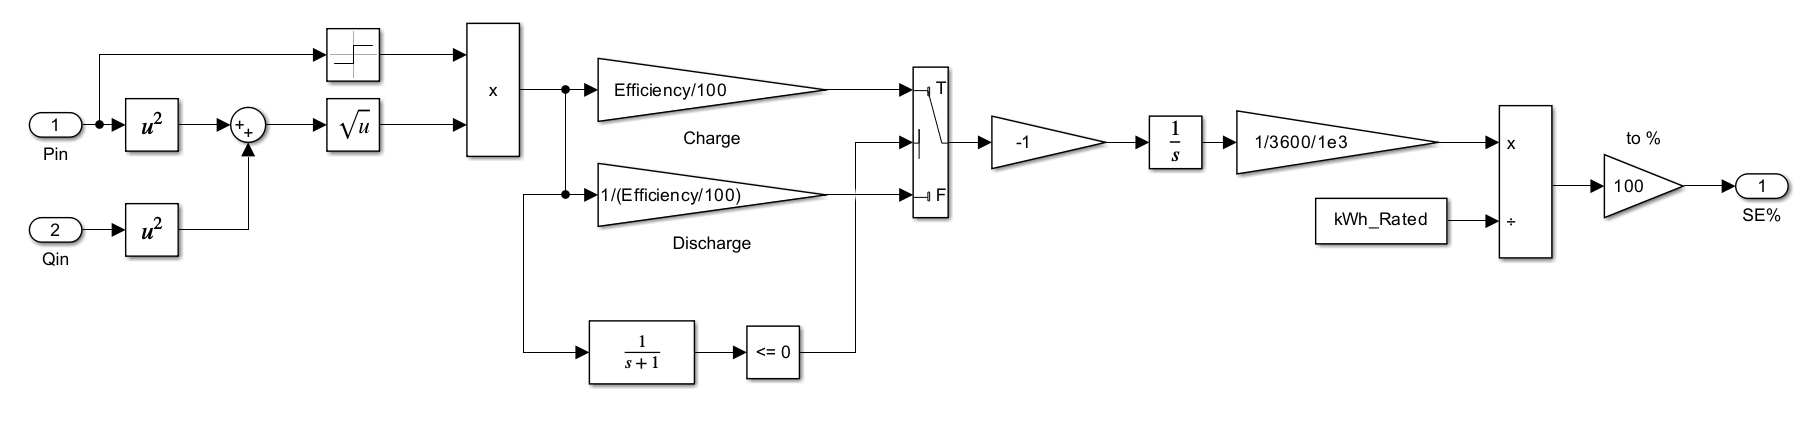
\includegraphics[width=12cm]{Abbildungen/SOC.png}
	\caption{Aufbau der SOC-Schätzung im Simulink Batteriemodell}\label{SOC}
\end{figure}

\paragraph{Dreiphasige Last als Umrichter}
Grundlegend wird in diesem Batteriemodell davon ausgegangen, dass die in der Steuerung festgelegte Leistung
innerhalb der Leistungsgrenzen aber unabhängig vom SOC oder sonstigen Faktoren, exakt an das Netz abgegeben werden kann.
Das ist eine starke aber notwendige Vereinfachung der tatsächlichen Gegebenheiten um überhaupt ein funktionierendes Modell
für diese Projektarbeit zu erstellen.
Durch diese Betrachtung ist es möglich die geforderte Leistung direkt an einen Simulink-Baustein zur dynamischen Last
anzuschließen. 
Ein wesentlicher Vorteil zeigt sich in diesem Baustein, durch die Möglichkeit sowohl negative als auch positive Leistung
an das Netz anzulegen.
Im Block zur Leistungssteuerung wird vorher die Ladeleistung der Batterie als positiv und die Entladeleistung als negativ definiert,
sodass beim Laden der Batterie tatsächlich eine Last am Netz anliegt und beim Entladen bekommt der dynamische Last-Baustein
ein negatives Signal und speist daher Leistung in das Netz ein.

Dieser Block findet seine Anwendung nur in der dreiphasigen Simulation aus Abschnitt~\ref{3phase}.
Da im bilanziellen Modell nur der Leistungsfluss betrachtet wird, braucht es keinen Batterieumrichter.

\subsection{Umsetzung Lade- und Entladestrategien}\label{Lade- und Entlade}
In diesem Abschnitt wird die Umsetzung der in Kapitel~\ref{Betriebsstrategien} beschriebenen Betriebsstrategien erklärt.
Da wir uns entschieden haben, die Batteriespeicher im Inselnetz für die Erbringung von FCR zu nutzen, lag es nahe 
die Deadband-Strategie zu implementieren.
Dafür wurde innerhalb des Simulink-Speicherblocks ein Subsystem erstellt, dass in Abbildung~\ref{Steuerung} zu sehen ist.

\begin{figure}[h!]
	\centering
	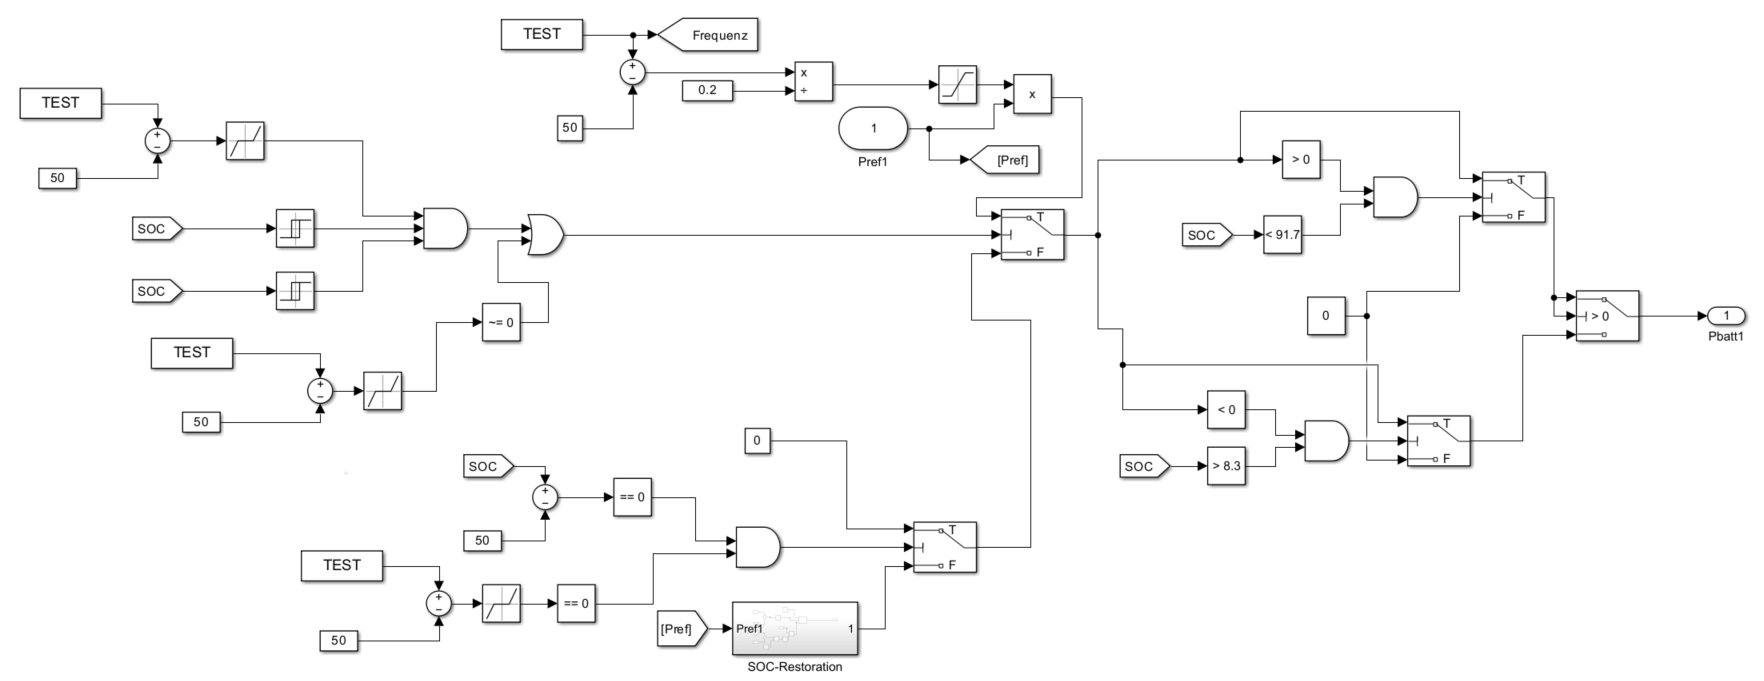
\includegraphics[width=14cm]{Abbildungen/Steuerung.png}
	\caption{Inhalt des Subsystems zur Leistungssteuerung der FCR-Batterie}\label{Steuerung}
\end{figure}

In der Mitte des Systems befindet sich ein Schalter der im Wesentlichen entscheidet ob Regelleistung bereitgestellt wird
oder der SOC der Batterie korrigiert wird.
Dafür werden zunächst mehrere Kriterien überprüft.
Der Schalter gibt den oberen Pfad zur FCR-Provision weiter wenn die Frequenzabweichung außerhalb des Totbandes von $\pm 10$ mHz liegt
und der SOC im erlaubten Arbeitsbereich von 35 \% bis 65 \% liegt.
Dieser Bereich ist durch die Übertragungsnetzbetreiber in \parencite[]{Reservebetrieb} festgelegt und ist abhängig vom Speicherverhältnis $\rho$.
Die Relays nach den SOC-Bausteinen schalten jeweils ab $8,3 \%$ und $91,7 \%$ ab, sodass der Speicher in einen Reservebetrieb wechselt wie er in \parencite[]{Reservebetrieb}
definiert ist.
Erst wenn der Ladezustand dann wieder im Arbeitsbereich liegt, geben die Relays frei und eine FCR-Erbringung ist möglich.
Zusätzlich ist eine Oder-Bedingung eingebaut, die den FCR-Zweig aktiv schaltet sobald die Frequenzabweichung $\pm 200$ mHz überschreitet.
Diese Maßnahme entspricht der Vorgabe zum gefährdeten Zustand, welcher ebenfalls in \parencite[]{Reservebetrieb} definiert 
und durch die Übertragungsnetzbetreiber vorgeschrieben ist.

Im oberen Schaltungszweig wird dann ie Abweichung der Frequenz von 50 Hz mit dem maximalen Wert von 0,2 Hz verglichen.
Ab diesem Wert soll die maximale Primärregelleistung ausgegeben werden wie in~\parencite[Kap. 3.1]{Regelleistung} gefordert.
Dafür wird das Ergebnis auf einen Wert zwischen -1 und 1 begrenzt und anschließend 
mit der maximalen Batterieleistung multipliziert.
Ab 200 Mhz wird also die volle Regelleistung erreicht, davor wird proportional zur Frequenzabweichung
weniger Leistung ausgegeben.

Ist keines der Kriterien erfüllt, gibt der Schalter den unteren Zweig zur SOC-Restoration frei.
Hier wird einmal überprüft ober überhaupt geladen werden muss ($SOC \neq 50 \%$) und ob geladen werden darf ($|\Delta f| < \pm 10 \text{mHz}$).
Erst wenn beide Kriterien erfüllt sind, gibt der Schalter den Wert aus dem Subsystem zur SOC-Restoration weiter.

\begin{figure}[h!]
	\centering
	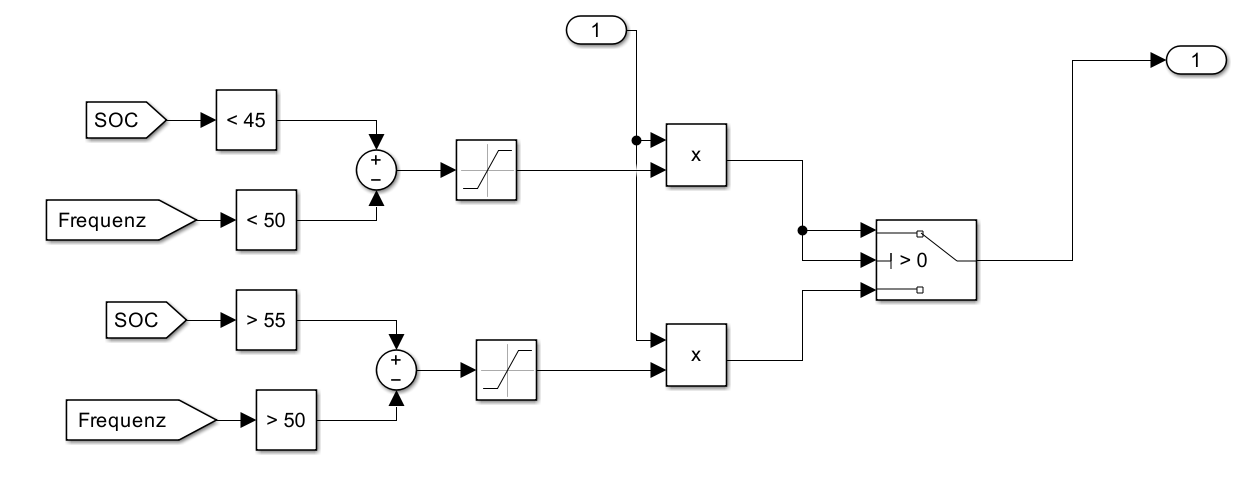
\includegraphics[width=12cm]{Abbildungen/SOC-Rest.png}
	\caption{Inhalt des Steuerblocks zur SOC-Restoration}\label{SOC-Rest}
\end{figure}

Abbildung~\ref{SOC-Rest} zeigt den Inhalt dieses Subsystems.
Es wird ein weiter Check durchgeführt ob der SOC tatsächlich eine Korrektur erfordert.
Die Leistung die dafür benötigt wird, berechnet sich hier aus der Abweichung des SOCs von 50 \%.
Dabei soll bei ca. 5 \% Ladezustand mit maximaler Leistung nachgeladen werden und bei einem Ladezustand von
90 \% möglichst schnell Leistung abgegeben werden.
Ein Saturation-Block begrenzt die Restorations-Geschwindigkeit dabei auf maximal 50 \% der vollen Batterieleistung.

\paragraph{Nachweis der Funktion}
Um die Funktion der Batteriesteuerung nachzuweisen wurde eine Simulation mit öffentlichen Frequenzdaten des europäischen Strromnetzes durchgeführt~\parencite[]{noauthor_netztransparenz_nodate}.
Um eine längere Simulation und Auswertung zu ermöglichen wurde das Batteriemodell vom Rest des Inselnetzes isoliert betrachtet.
Während der Simulation mit den sekündlichen Frequenzwerten wurde der SOC und die Leistung der Batterie aufgezeichnet.

\begin{figure}[h!]
	\centering
	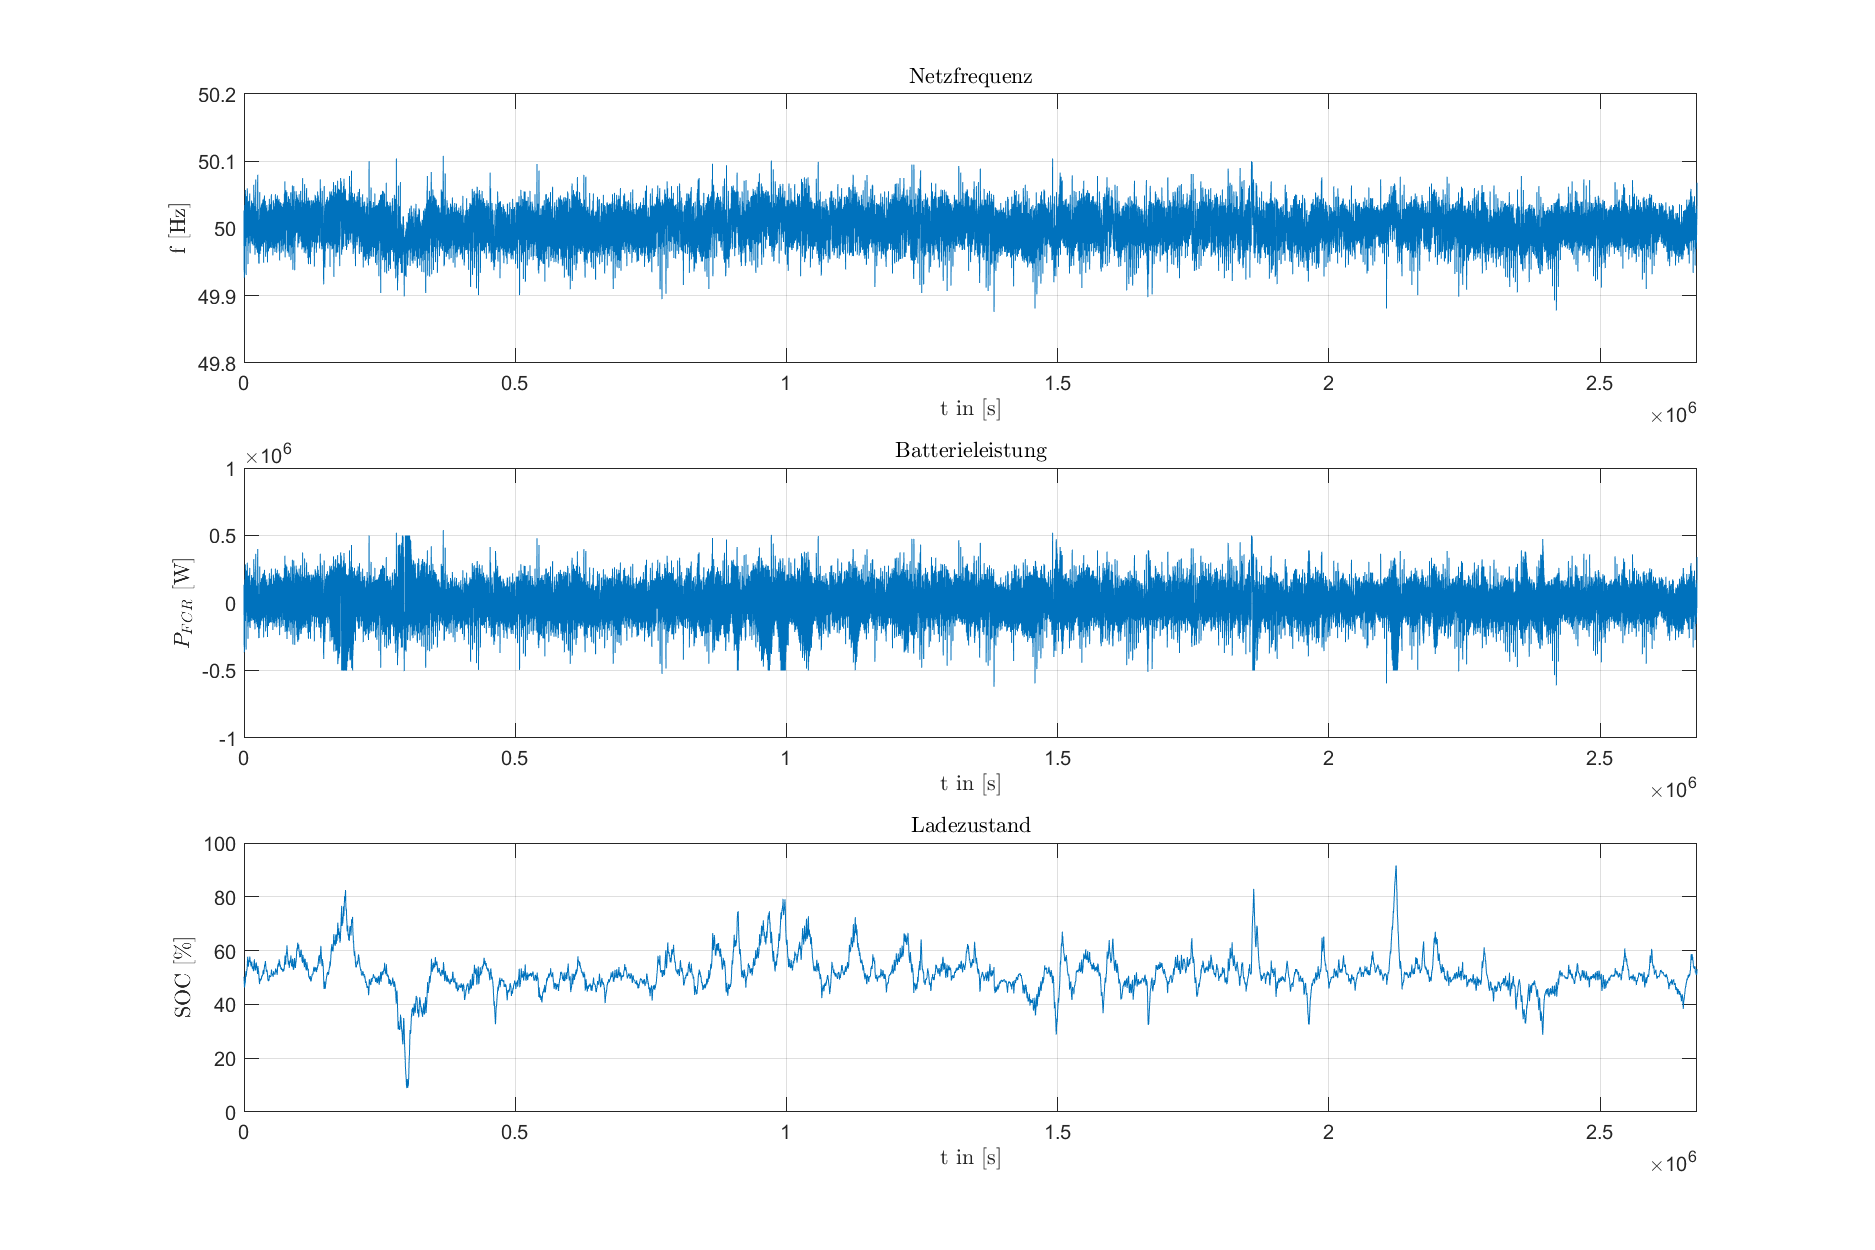
\includegraphics[width=14cm]{Abbildungen/SteuerungFCR.png}
	\caption{Messergebnisse der Simulation mit vorgegebenen Frequenzwerten}\label{FCRMessung}
\end{figure}

Abbildung~\ref{FCRMessung} zeigt den Gesamten Verlauf der Messreihe.
Die Simulation ging dabei über einen Zeitraum von 31 Tagen und wurde mit den Frequenzdaten vom Dezember 2023 durchgeführt.
Der Speicher wurde mit einer Kapazität von $1$ MWh und einer Leistung von $1$ MW modelliert.
Daraus ergibt sich ein Speicherverhältnis von $\rho = 1h$, was der Dimensionierung des Beispielszenarios aus\parencite[S. 7]{Reservebetrieb}
entspricht.

Im Verlauf des Ladezustands zeigt sich, dass der Speicher über den ganzen Monat genug Reserve bereitstellen kann.
Die kurzen Phasen mit geringer Frequenzabweichung genügen um einen nötigen Reservebetrieb weitestgehend zu vermeiden.
Dazu ist allerdings zu erwähnen, dass während des gesamten Monats keine Differenz außerhalb der $\pm$ 200 Mhz Grenze erreicht wird
und daher kein gefährdeter Zustand nötig wird.

\begin{figure}[h!]
	\centering
	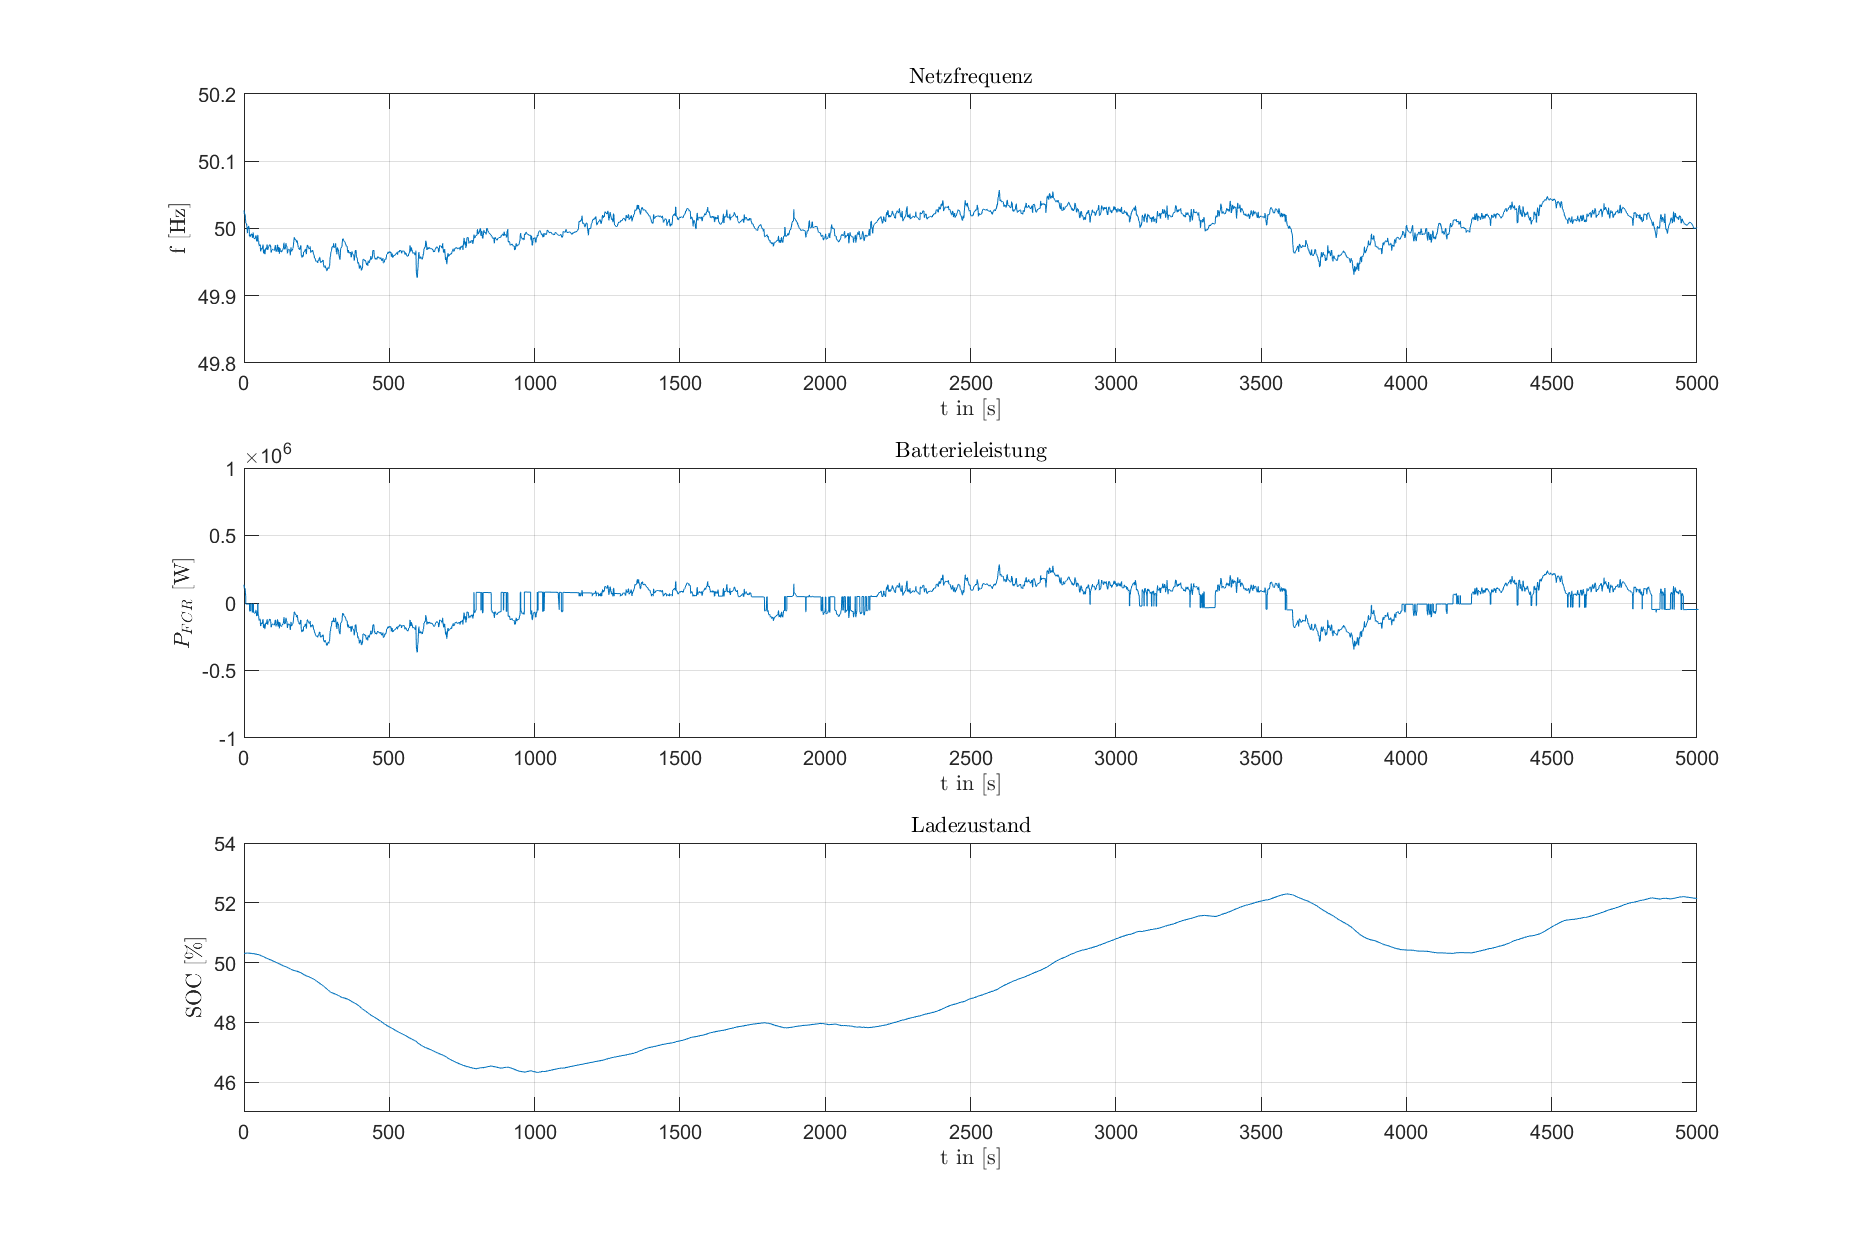
\includegraphics[width=14cm]{Abbildungen/SteuerungFCR2.png}
	\caption{Ausschnitt aus den Messergebnissen der Simulation mit vorgegebenen Frequenzwerten}\label{FCRMessung2}
\end{figure}

Abbildung~\ref{FCRMessung2} zeigt einen Ausschnitt aus dem Gesamtverlauf.
Hier ist deutlich zu erkennen, dass der Batteriespeicher bei einer Frequenzabweichung von über $\pm$ 10 mHz
anfängt FCR bereitzustellen.
Dabei folgt er der Höhe der Frequenzabweichung proportional. 
Zwischen diesen Phasen wird der SOC entsprechend regeneriert.

\begin{figure}[h!]
	\centering
	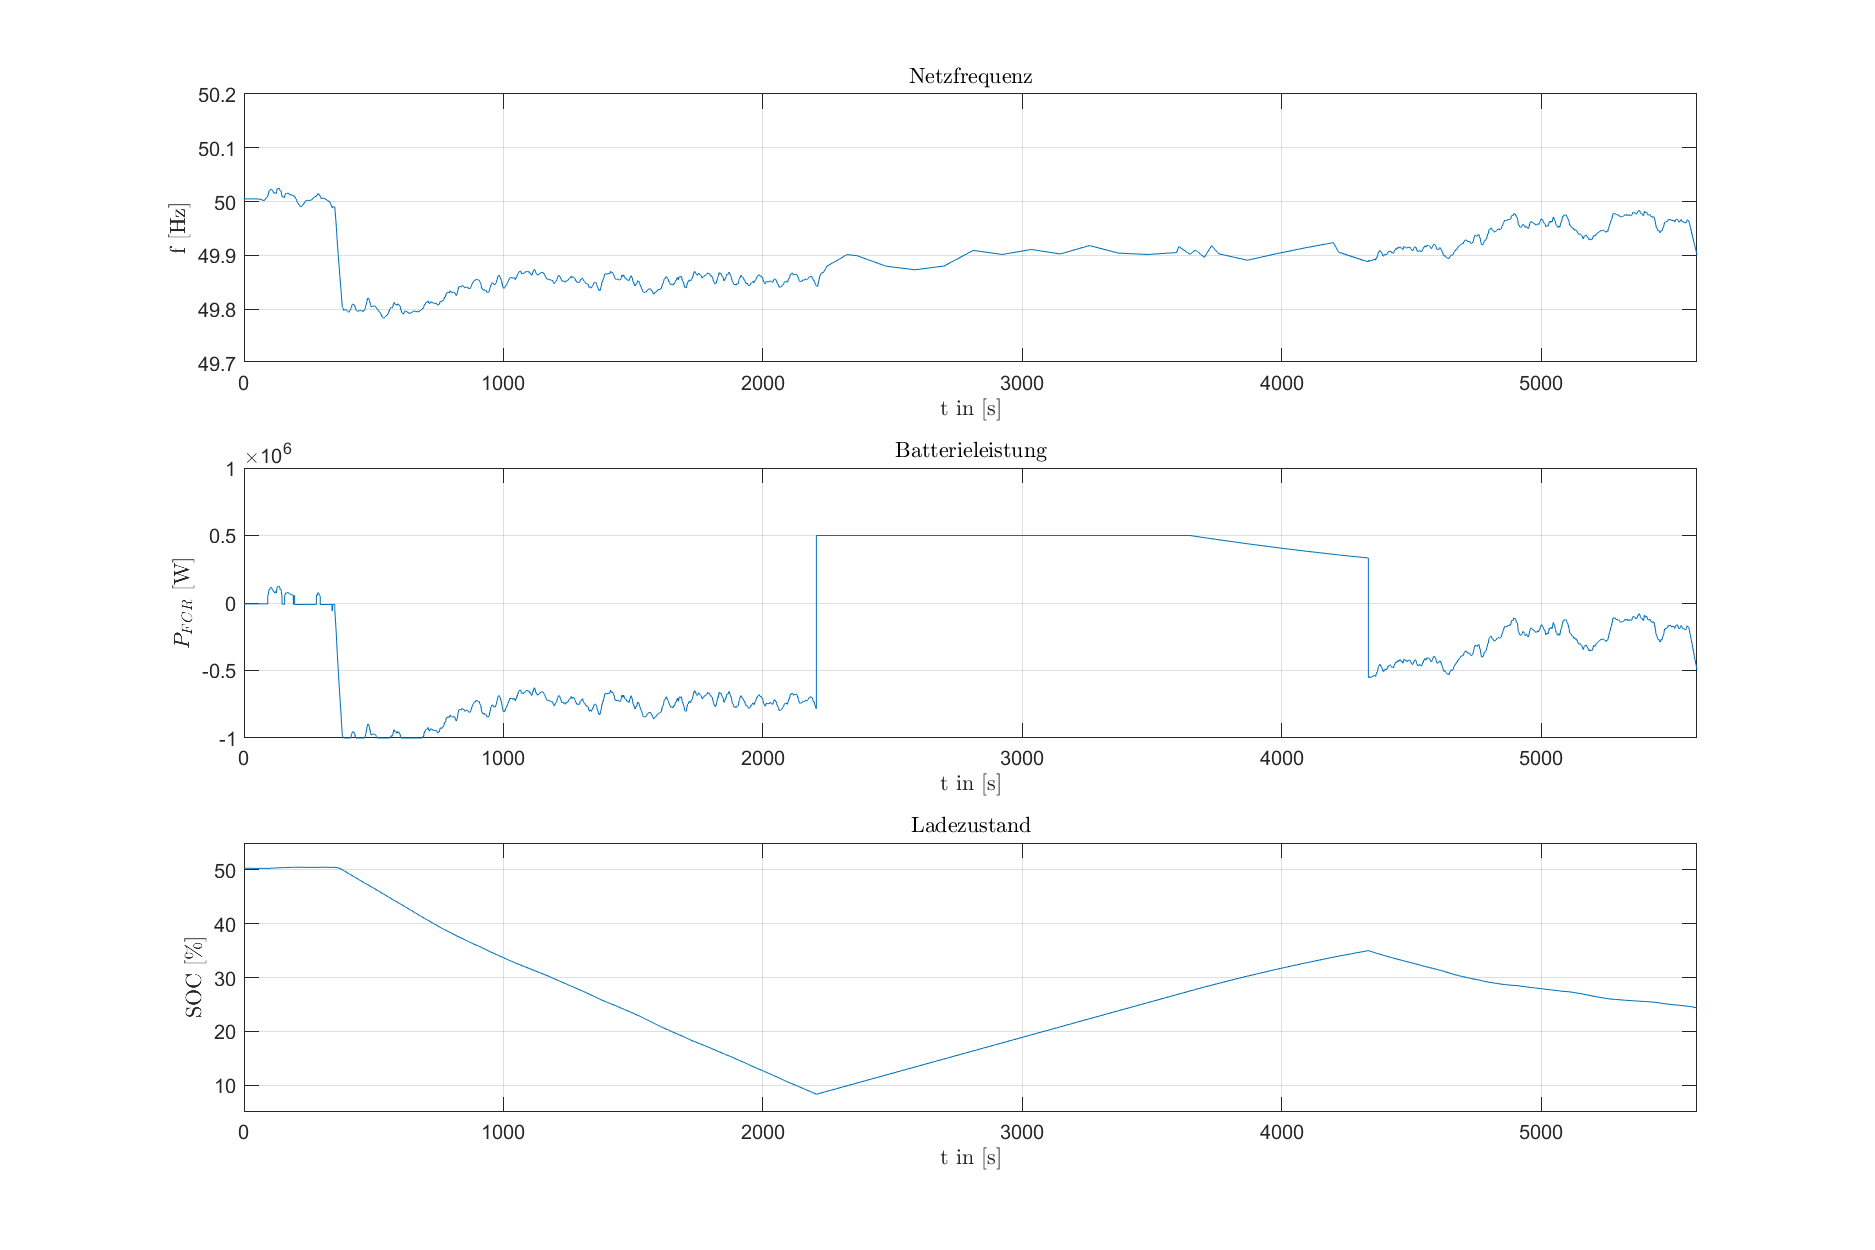
\includegraphics[width=14cm]{Abbildungen/SteuerungFCR3.png}
	\caption{Simulation mit Beispielszenario der Übertragungsnetzbetreiber}\label{FCRMessung3}
\end{figure}

Um das Verhalten und die Übergänge im gefährdeten Zustand dennoch zu überprüfen wurde die Simulation mit den Frequenzdaten
des Beispielszenarios der Übertragungsnetzbetreiber aus~\parencite[]{Reservebetrieb} wiederholt.
Abbildung~\ref{FCRMessung3} zeigt die dabei aufgezeichneten Verläufe.

Bei knapp 300 s bricht die Frequenz hierbei auf ca. 49,8 Hz ein.
Der FCR-Speicher muss dabei in den gefährdeten Zustand wechseln und innerhalb weniger Sekunden
die maximale Leistung zur Verfügung stellen.
Im Verlauf der Batterieleistung sieht man, dass ohne Verzögerung 1 MW Leistung angelegt wird.
Der SOC sinkt dabei drastisch und erreicht nach ungefähr 30 min die Grenze für den Reservebetrieb.
Ab diesem Zeitpunkt wird die FCR-Provision unterbrochen und die Batterie lädt sich mit $500$ kW 
bis zum Erreichen des erlaubten Arbeitsbereichs bei $35 \%$.
Laut Vorgabe der Übertragungsnetzbetreiber darf dieses Nachladen maximal 2 Stunden dauern.
Der Speicher in dieser Simulation braucht etwas über eine halbe Stunde und kann anschließend wieder
Regelleistung zur Verfügung stellen.



\section{Netzmodell}
\section{Netzmodell}

Zur Untersuchung der Inselnetze werden die zuvor gezeigten Teilmodelle zu Netzmodellen verschaltet. Abhängig von der geforderten Modelltiefe und dem geforderten Detailgrad, stehen grundsätzlich drei verschiedene Simulationsmethoden in Simulink zur Verfügung. Im folgenden werden diese drei Methoden kurz beleuchtet und anschließend eine Entscheidung für die nachfolgenden Modelle begründet.

\textbf{Bilanzmodell}

Das Bilanzmodell stellt die oberflächlichste Betrachtung dar und dient zur Betrachtung der Leistungsbilanz im Inselnetz. Hierfür werden die einzelnen Komponenten vereinfacht dargestellt und elektrische Parameter des Netzes vernachlässigt. Durch diese Vereinfachungen ergeben sich kurze Simulationszeiten, weshalb es möglich ist lange Zeiträume zu betrachten. Jedoch bildet dieses Modell mit steigender Vereinfachung immer weniger die Realität ab, wodurch sich dieses Modell besonders für grobe Betrachtungen anbietet.

\textbf{Momentanwertsimulation (EMT)}

Bei der Momentanwertsimulation unter Berücksichtigung von elektromagnetischen Transienten wird das Netz durch die jeweiligen dreiphasigen Netzzweige beschrieben. Hierdurch ergibt sich ein Gleichungssystem aus Differentialgleichungen, welches für jeden betrachteten Zeitschritt gelöst wird. Somit lassen sich Netze auch in unsymmetrischen Netzzuständen und sehr Detailgetreu hinsichtlich ihrer elektrischen Eigenschaften beschrieben. Der Rechenaufwand ist hier jedoch vergleichsweise hoch und steigt mit der Komplexität des betrachteten Netzes. \cite{Simulationsmethoden}

\textbf{Raumzeigersimulation (RMS)}

Eine etwas weniger detaillierte Simulationsmethode stellt die Raumzeigersimulation dar. Hierbei werden die bei der Momentanwertssimulation betrachteten elektromagnetischen Vorgänge vernachlässigt, wodurch sich eine deutlich weniger rechenintensive Simulation ergibt. Dennoch ist dieses Modell detailliert genug, um Spannungs- oder Frequenzregelung in Energienetzen zu untersuchen. Statt den tatsächlichen Sinusverlauf der dreiphasigen Wechselspannungen zu betrachten, werden diese als Vektoren in einem rotierenden Koordinatensystem dargestellt. Das Koordinatensystem rotiert hierbei mit der Netzfrequenz, wodurch sich ein stehender Zeiger ergibt, der auch Raumzeiger genannt wird und aus den Komponeten d und q besteht. Dies ermöglicht deutlich größere SImulkationsschritte, da der Sinus nicht mehr exakt nachgebidlet werden muss. Jedoch wird nach Modell auch unegnauer mit steigender Abweichung der Netzfrequernz von der Frequenz des drehenden Koordinatensystems. \cite{Simulationsmethoden}

Nach kurzer Betrachtung der drei Simulationsmethoden werden im folgenden die bilanzielle und die Betrachtung mithilfe eines Raumzeigers verfolgt, da beide Modelle eine akzeptable Simulationsdauer und -tiefe bieten. Das bilanzielle Modell dient hier eher der groben Betrachtung und das Raumzeigermodell der Frequenzbetrachtung. Das Momentanwertsmodell scheidet durch den hohen Simulationsaufwand und die Detailtiefe aus. Die zuvor beschriebenen Modelle der Erzeuger, Verbraucher und Speicher ermöglichen durch die ihre starke Vereinfachung keine detaillierte Betrachtung der elektrischen Eigenschaften.

\subsection{Bilanziell}

Sinn und Zweck des bilanziellen Modells ist es die Situation zwischen Erzeugung und Verbrauch im Inselnetz über lange Zeiträume zu untersuchen. Somit ist es möglich den Energiespeicher auszulegen und mögliche kritische Zeitpunkte zu identifizieren. Wie es der Name vermuten lässt, handelt es sich hierbei um eine bilanzielle Betrachtung zwischen Erzeugung und Verbrauch. Die dabei entstehende Diskrepanz wird mithilfe des Energiespeichers abgefangen, indem dieser Systemdienlich überschüssige Energie aufnimmt oder gespeicherte Energie abgibt. \autoref{fig:Bilanziell} zeigt die oberste Ebene und somit den groben Aufbau des Modells.

\begin{figure}[H]
	\centering
	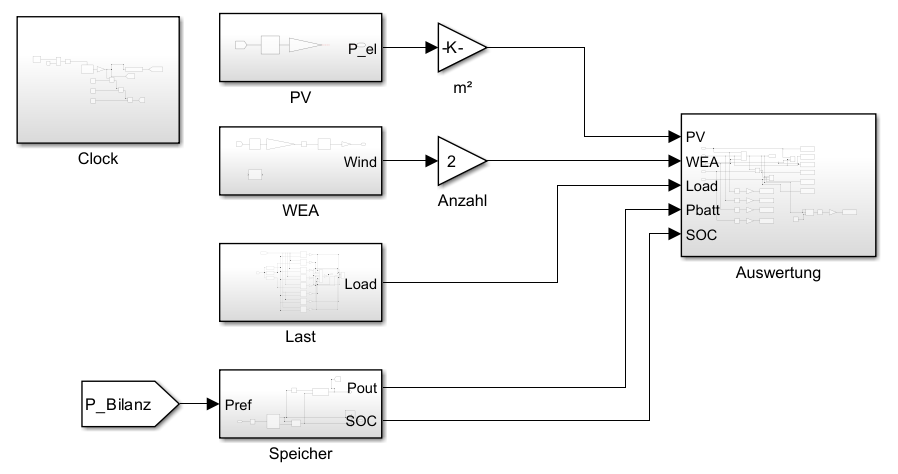
\includegraphics[width=0.9\linewidth]{Abbildungen/Bilanziell.png}
	\caption{Bilanzielles Modell eines Inselnetzes in Matlab/Simulink}
	\label{fig:Bilanziell}
\end{figure}

Die Erzeuger, Speicher und Verbraucher sind analog zu den vorherigen Erklärungen aufgebaut. Es wird angenommen, dass der Speicher exakt die Menge an Energie aufnimmt oder abgibt, welche das System benötigt. Dabei hält er jedoch seine vorgegebenen Grenzen hinsichtlich Kapazität, maximaler Leistung und SOC ein. Das Subsystem Clock dient als Taktgeber für alle Komponenten und ermöglicht es das Modell in beliebigen Zeitschritten simulieren zu lassen. 
%Der Aufbau ist in \autoref{fig:clock} zu sehen.

\begin{figure}[H]
	\centering
	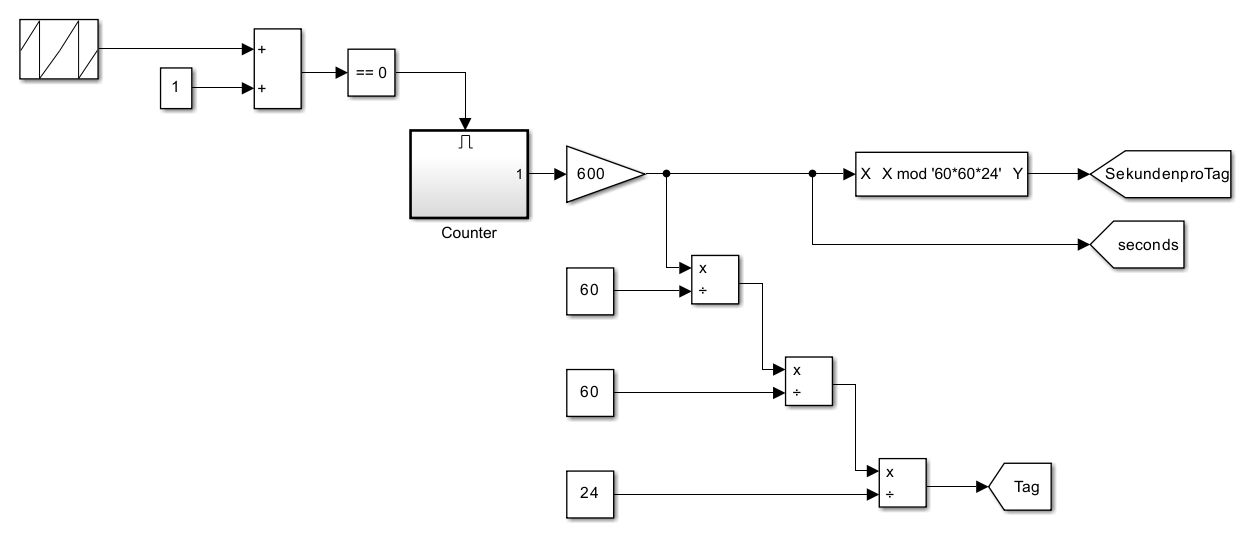
\includegraphics[width=0.9\linewidth]{Abbildungen/Clock.png}
	\caption{Taktgeber für das bilanzielle Modell}
	\label{fig:clock}
\end{figure}

Der Batteriespeicher erhält die Leistungsbilanz ohne Energiespeicher als Eingangsgröße und berechnet hieraus die ein- oder auszuspeisende Leistung. Diese wird wieder mit der zuvor berechneten Leistungsbilanz des Inselnetzes ohne Speicher verrechnet, wodurch sich der Verlauf der Bilanz unter Verwendung eines Speichersystems ergibt. Diese Auswertung wird in dem gleichnamigen Subsystem vorgenommen, welches in \autoref{fig:Auswertung} dargestellt ist.

\begin{figure}[H]
	\centering
	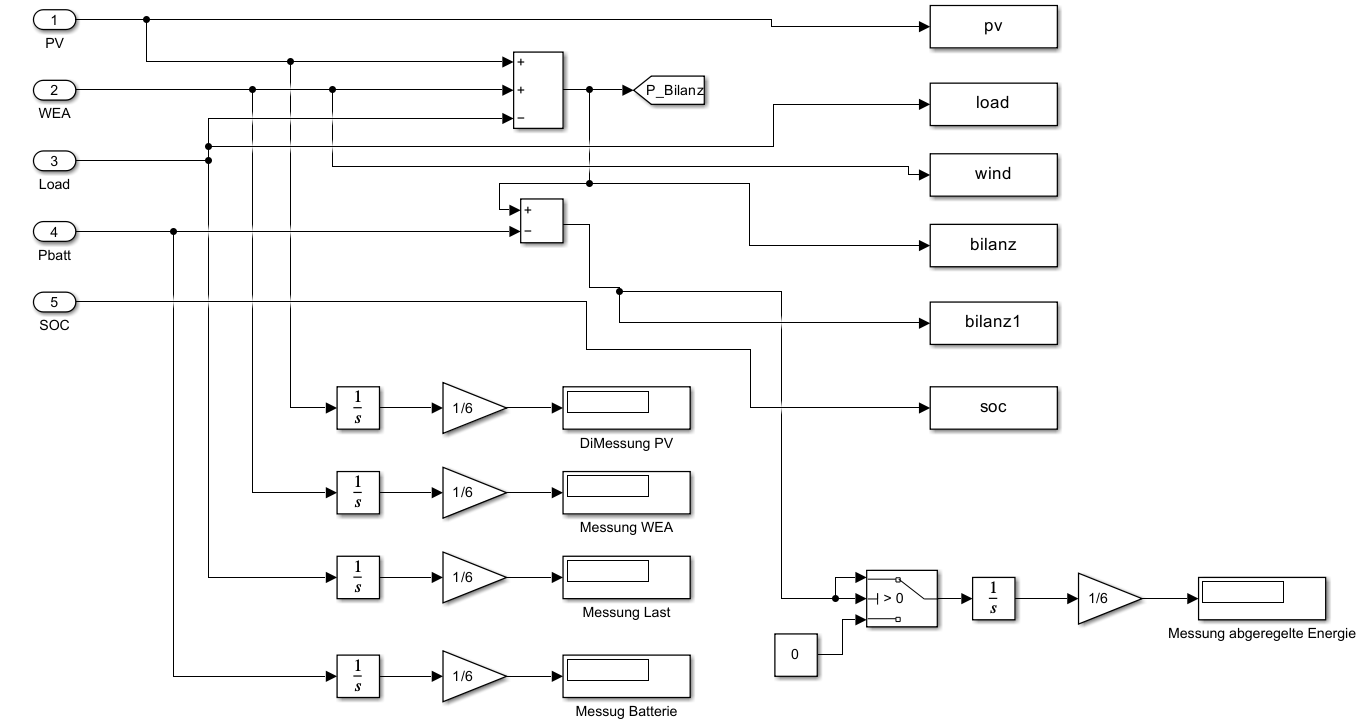
\includegraphics[width=0.9\linewidth]{Abbildungen/Auswertung.png}
	\caption{Auswertung der einzelnen Komponenten im bilanziellen Modell}
	\label{fig:Auswertung}
\end{figure}

Zusätzlich erfolgt eine Energiemessung der einzelnen Komponenten, um hier eine weitere Auswertung vornehmen zu können.

\subsection{Dreiphasig}\label{3phase}
Um das Frequenzverhalten des Inselnetzes so gut es geht auszuwerten wurde ein dreiphasiges Simulink-Modell aufgebaut.
Dabei wurde auf eine Vorlage zurückgegriffen welche anschließend an das geplante Inselnetz angepasst wurde.
Die Frequenzmessung konnte dabei nur mit einem Diesel-Generator verlässlich umgesetzt werden, woraus sich ein paar Probleme ergeben
die im Folgenden Abschnitt genauer erklärt werden.
Das in~\ref{Speicher} eingeführte Speichermodell zur FCR-Erbringung wurde für diese Simulation ebenfalls genutzt.

\begin{figure}[h!]
	\centering
	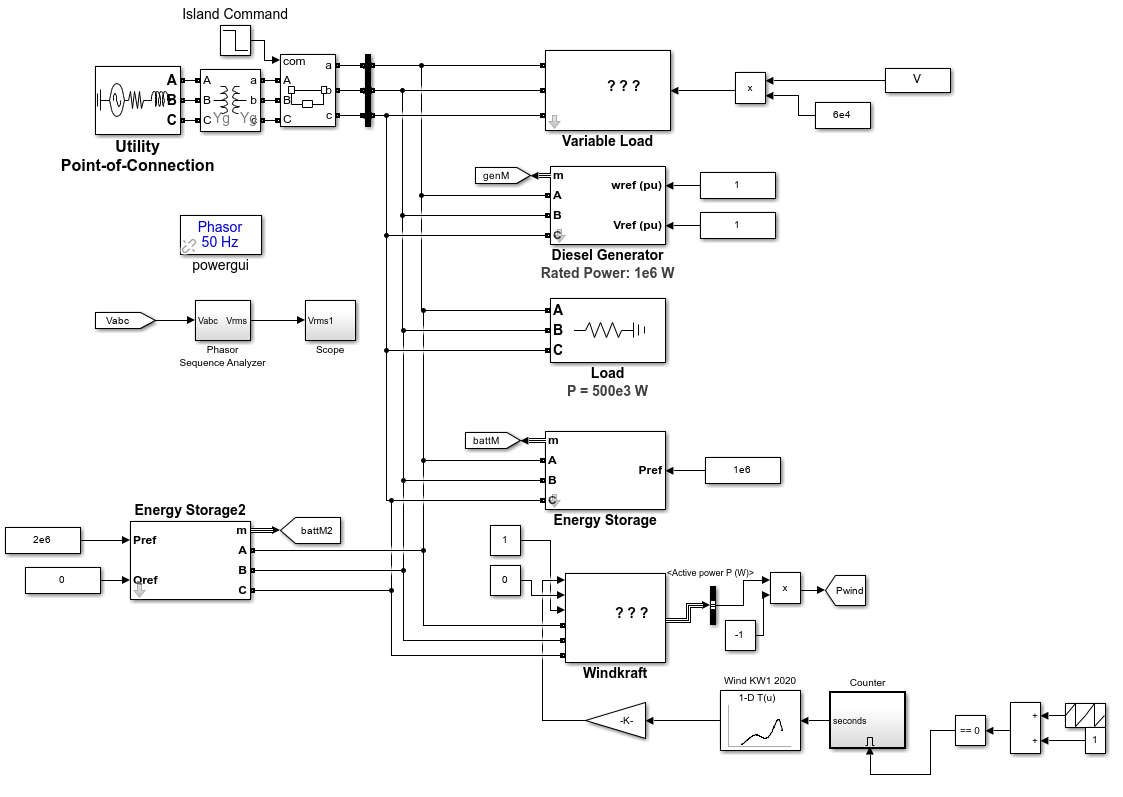
\includegraphics[width=14cm]{Abbildungen/Dreiphasig.png}
	\caption{Dreiphasiges Simulink-Modell eines Inselnetzes}\label{Mod:3phase}
\end{figure}

Abbildung~\ref{Mod:3phase} zeigt das gesamte Simulink-Modell mit allen Komponenten.
Um eine Auswertung der Dreiphasen-Spannung und Frequenz zu ermöglichen mussten alle Berechnungen als kontinuierliche Zeiger-Simulation 
durchgeführt werden.
Der Rechenaufwand im Vergleich zu diskreten Simulationen ist dabei deutlich erhöht was uns nur eine eingeschränkte
Auswertung im Bereich weniger Stunden erlaubte.

\paragraph{Komponenten des Modells}
Als Erzeuger für das hier simulierte Inselnetz dient in erster Linie die Windkraftanlage die bereits in Abschnitt~\ref{Erzeuger} beschrieben wurde.
Zusätzlich speist der Diesel-Generator, über den die Frequenz gemessen wird, das Inselnetz mit Leistung.
Um diese zusätzlich erbrachte Leistung etwas auszugleichen, wurde eine feste Last von 500 kW eingesetzt.

Der tatsächliche Verbrauch des Inselnetzes wurde als variable Last umgesetzt.
Diese Last wird mit den Profilen aus Abschnitt~\ref{Verbraucher} gespeist und gibt den entsprechenden Verbrauch ans das Inselnetz
weiter.

Um einen stabilen Anlauf des Inselnetzbetriebs zu ermöglichen ist das Netz zunächst an eine konstante Dreiphasen-Stromquelle 
angeschlossen. 
So wird das Netz die ersten 15 s mit 50 Hz Spannung gespeist bevor die Spannungsquelle getrennt wird und das Netz 
eigenständig läuft.

Zusätzlich zu dem FCR-Speichermodell ist ein weiterer Speicher implementiert der die Differenz zwischen erzeugter 
Leistung der Windkraftanlage und verbrauchter Leistung der Lastprofile ausgleicht.
Die Speichersteuerung reagiert dabei auf die Differenz zwischen aktuell erzeugter Windenergie und prognostiziertem Verbrauch.
Dabei können sowohl die realen Profile der Verbraucher eingesetz werden als auch leicht veränderte um Fehler in der Prognose zu simulieren.
Der entsprechende Speicher wurde mit 2 MW Leistung und einer Kapazität von 2MWh dimensioniert.
Für einen dauerhaften Betrieb wäre ein deutlich größerer Speicher nötig allerdings konnte in dieser Simulation
ein Einbruch der Frequenz durch das Abschalten des Speichers untersucht werden und damit die korrekte Funktion des FCR-Speichers.

\paragraph{Umsetzung der Frequenzmessung}
Um die Momentan-Frequenz des Inselnetzes zu überwachen wurde verschiedene Maßnahmen untersucht.
Zum einen wurde eine Methode namens Zero Crossing Counts in Erwägung gezogen.
Simulink bieten dafür einen fertigen Baustein, welche die Nulldurchgänge eines Signals zählt und als aktuellen Wert ausgibt.
Teilt man nun die Anzahl der Nulldurchgänge durch die Simulationszeit, lässt sich die Frequenz des jeweiligen Signals bestimmen.
Diese Frequenz ist allerdings als Mittelwert zu verstehen.
Kurzfristige Schwankungen werden mit zunehmender Simulationszeit kaum berücksichtigt und ein genauer Wert der aktuellen
Netzfrequenz ist so nicht darstellbar.

Eine weitere Option basiert auf einem Simulink-Baustein namens Sequence Analyzer. 
Dieser wird in der Simulation schon genutzt um die Amplitude der Netzspannung zu bestimmen.
Zusätzlich kann dieser Block auch die Phase der Dreiphasen-Spannung ausgeben.
Die Änderung dieser Phasen wird mit einem rotierenden Zeiger bei 50 Hz verglichen und eine aktuelle Signalfrequenz kann bestimmt werden.

Auch nach langer Fehlersuche konnten wir mit dieser Methode leider keine eindeutige Frequenzmessung umsetzen.
Schon relativ geringe Schwankungen der Netzfrequenz führten bei allen Versuchen dazu, dass die so berechnete Frequenz
ausriss und sich teilweise bei Werten um $-500 Hz$ einstellte.

Letztendlich mussten wir uns auf Grund des begrenzten Zeitrahmens für diese Projektarbeit dafür entscheiden die Frequenzmessung
doch über den Synchrongenerator umzusetzen.

Dabei wird die Frequenz des Generators selber gemessen.
Da dieser synchron mit dem Netz gekoppelt ist entspricht diese in etwa auch der Netzfrequenz.
Dabei ist allerdings das Trägheitsverhalten des Generators selber zu beachten.
Durch die Massenträgheit ist der Frequenzverlauf des Generators deutlich geglättet.
Durch die Bereitstellung von Momentanreserve werden kleinere Schwankungen quasi direkt vom Generator ausgeglichen.
Der FCR-Speicher kommt in dieser Simulation daher nur eingeschränkt zum Einsatz.



\chapter{Auswertung}

\section{Bilanziell}




\subsection{Szenario Standort Bremen}

Dieses Szenario betrachtetet ein Ins

Um die Gesamtlast realitätsnah zu gestalten, werden die Gewichtungsfaktoren an die Anteile der Verbrauchergruppen am Nettostromverbrauch in Deutschland für das Jahr 2023 angelehnt. Die Verteilung der Verbräuche ist in \autoref{fig:pie} dargestellt.

\begin{figure}[H]
	\centering
	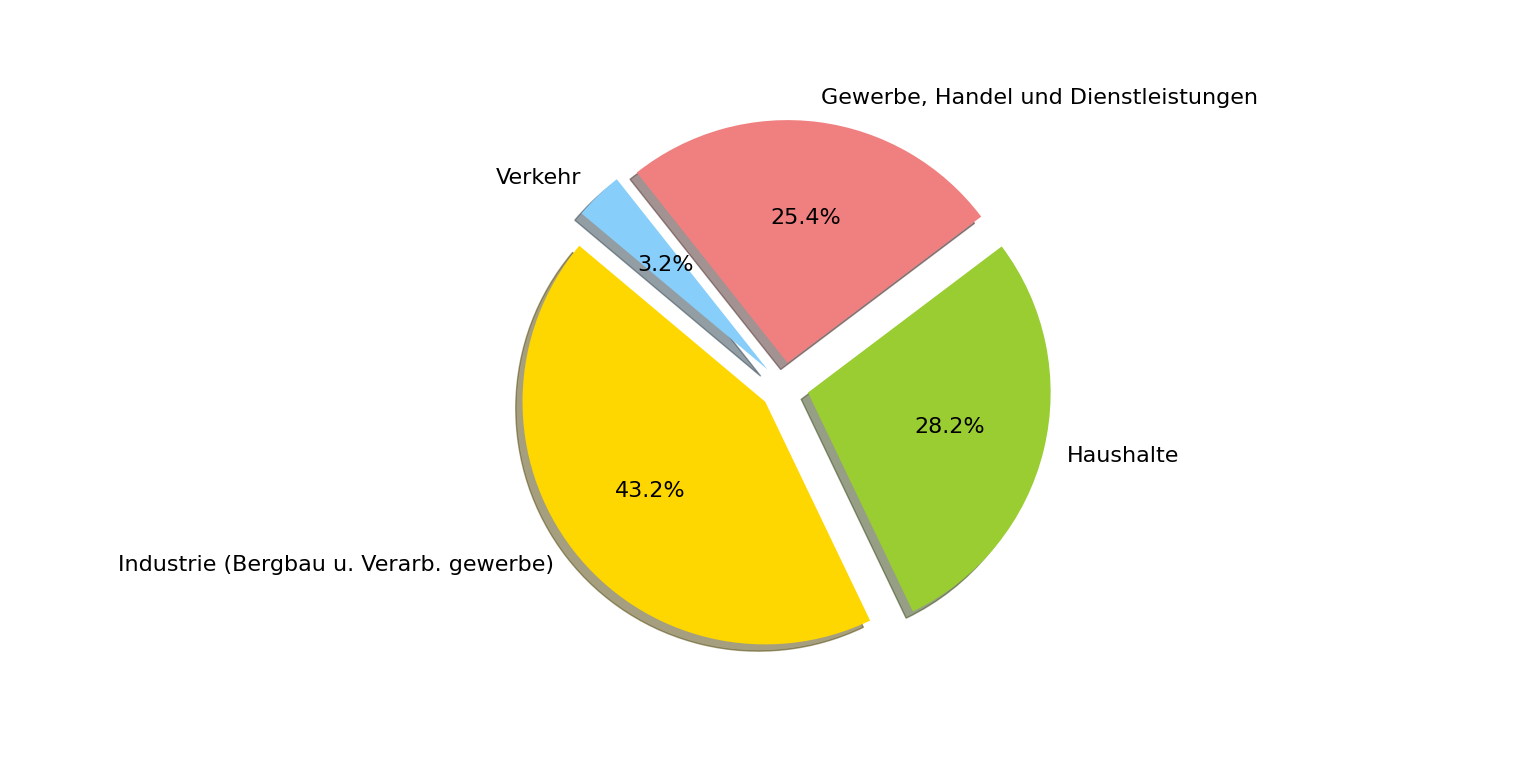
\includegraphics[width=0.8\linewidth]{Abbildungen/Stromverbrauch.png}
	\caption{Anteile der Verbrauchergruppen am Nettostromverbrauch 2023}
	\label{fig:pie}
\end{figure}

Da sich die jeweiligen Verbrauchergruppen aus diversen Lastprofilen zusammensetzen, werden die vorhandenen Lastprofile bestmöglich Gewichtet, um möglichst der Realität zu entsprechen. Es wird eine folgende Gewichtung der Lastprofile gewählt:

\begin{center}
	\begin{tabular}[htpb]{c|c}
		\textbf{Lastkurve} & \textbf{Gewichtung} \\
		\hline
		H0 Haushalt & 25~\% \\
		W0 Wärmepumpe & 5~\% \\
		G4 Friseur & 6~\% \\
		G5 Bäckerei & 7~\% \\
		S0 Straßenbeleuchtung & 1~\% \\
		L0 Landwirtschaft & 6~\% \\
		G3 Gewerbe durchlaufend & 25~\% \\
		G1 Werktags & 25~\% 
	\end{tabular}
\end{center}

Dies stellt lediglich eine Vereinfachung dar und spiegelt keinesfalls die Realität wieder. \autoref{fig:Gesamtlast} zeigt das resultierende Gesamtastprofil für einen Tag und normiert auf $1000~kWh/a$.

\begin{figure}[H]
	\centering
	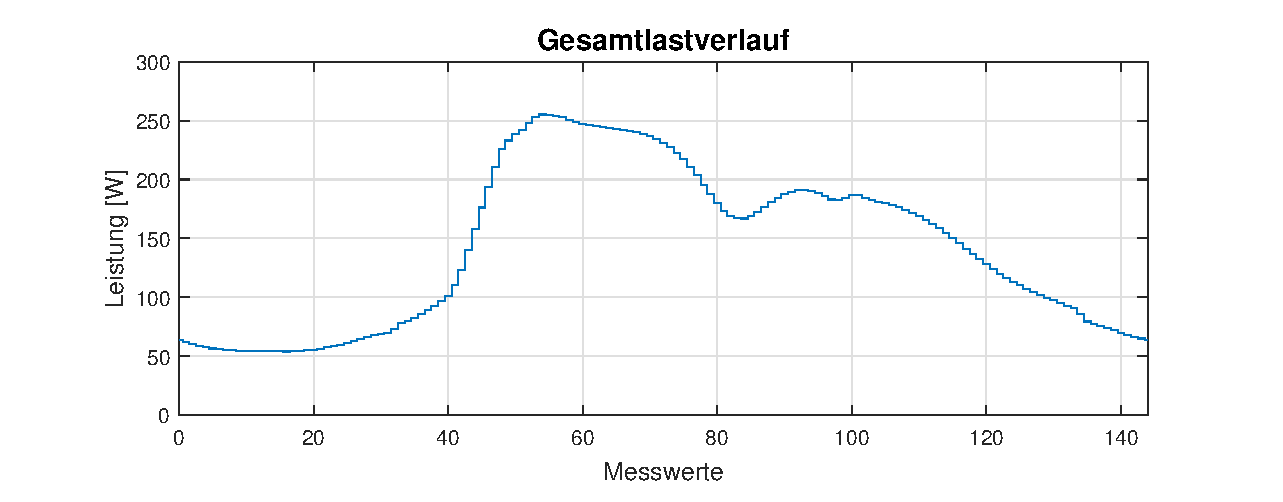
\includegraphics[width=0.8\linewidth]{Abbildungen/Gesamtlast.eps}
	\caption{Kombiniertes Gesamtlastprofil für einen Werktag im Winter}
	\label{fig:Gesamtlast}
\end{figure}

\subsection{Szenario Helgoland}

Für dieses Szenario dient die Insel Helgoland als Grundlage für Wetter und Verbrauchsdaten. Da es sich bei Helgoland, um die letzte ans Stromnetz angeschlossene Gemeinde handelt und die Insel weit entfernt von der Küste liegt, bietet diese eine realistisches Szenario für ein Inselnetz.

\autoref{fig:helgolandVerbrauch} zeigt den jährlichen Stromverbrauch auf der Insel Helgoland für das Jahr 2008. Der Gesamtverbrauch beträgt hier $11,6~GWh/a$.

\begin{figure}[H]
	\centering
	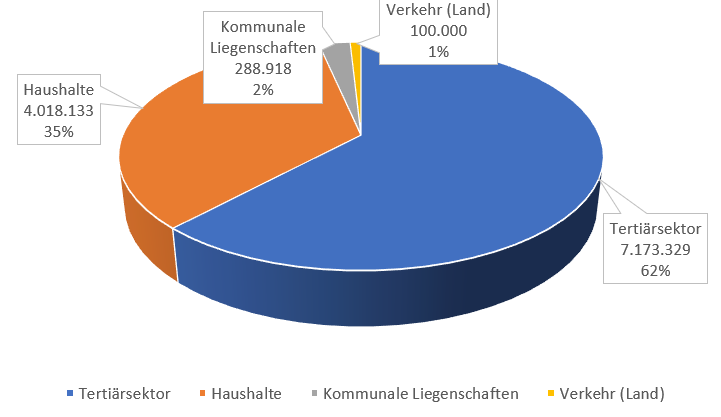
\includegraphics[width=0.6\linewidth]{Abbildungen/StromverbrauchHelgoland.png}
	\caption{Elektrische Energie [kWh/a] und prozentualer Anteil nach Sektoren im Jahr 2008 nach \cite{Helgoland}}
	\label{fig:helgolandVerbrauch}
\end{figure}

Besonders stechen hier der hohe Anteil an Haushalten heraus. Zudem besitzt Helgoland keine eigene Landwirtschaft und durch die touristische Auslegung wird von einem betrieb am Wochenende ausgegangen. Zur Nachbildung dieses Verbraucherprofils wird die folgende Gewichtung von Standardlastprofilen verwendet.

\begin{center}
	\begin{tabular}[htpb]{c|c}
		\textbf{Lastkurve} & \textbf{Gewichtung} \\
		\hline
		H0 Haushalt & 35~\% \\
		W0 Wärmepumpe & 5~\% \\
		G4 Friseur & 7~\% \\
		G5 Bäckerei & 7~\% \\
		S0 Straßenbeleuchtung & 1~\% \\
		L0 Landwirtschaft & 0~\% \\
		G3 Gewerbe durchlaufend & 30~\% \\
		G1 Werktags & 15~\% 
	\end{tabular}
\end{center}

In diesem Szenario werden die Wetterdaten der Wetterstation auf Helgoland aus dem Jahr 2020 verwendet, da diese Daten wenig Messfehler beinhalten. Zur Deckung der genannten Last wird eine Windenergieanlage mit einer Spitzenleistung von 3~MW verwendet. Zudem stehen nach \cite{Helgoland} ca. 11.130~m² Dachflächen für die Nutzung von Photovoltaikanlagen zur Verfügung. 

Wird nun das Jahr 2020 simuliert, ergeben sich für das Energiesystem ohne Speicher die Verläufe in \autoref{fig:helgolandVerlaufOhne}.

\begin{figure}[H]
	\centering
	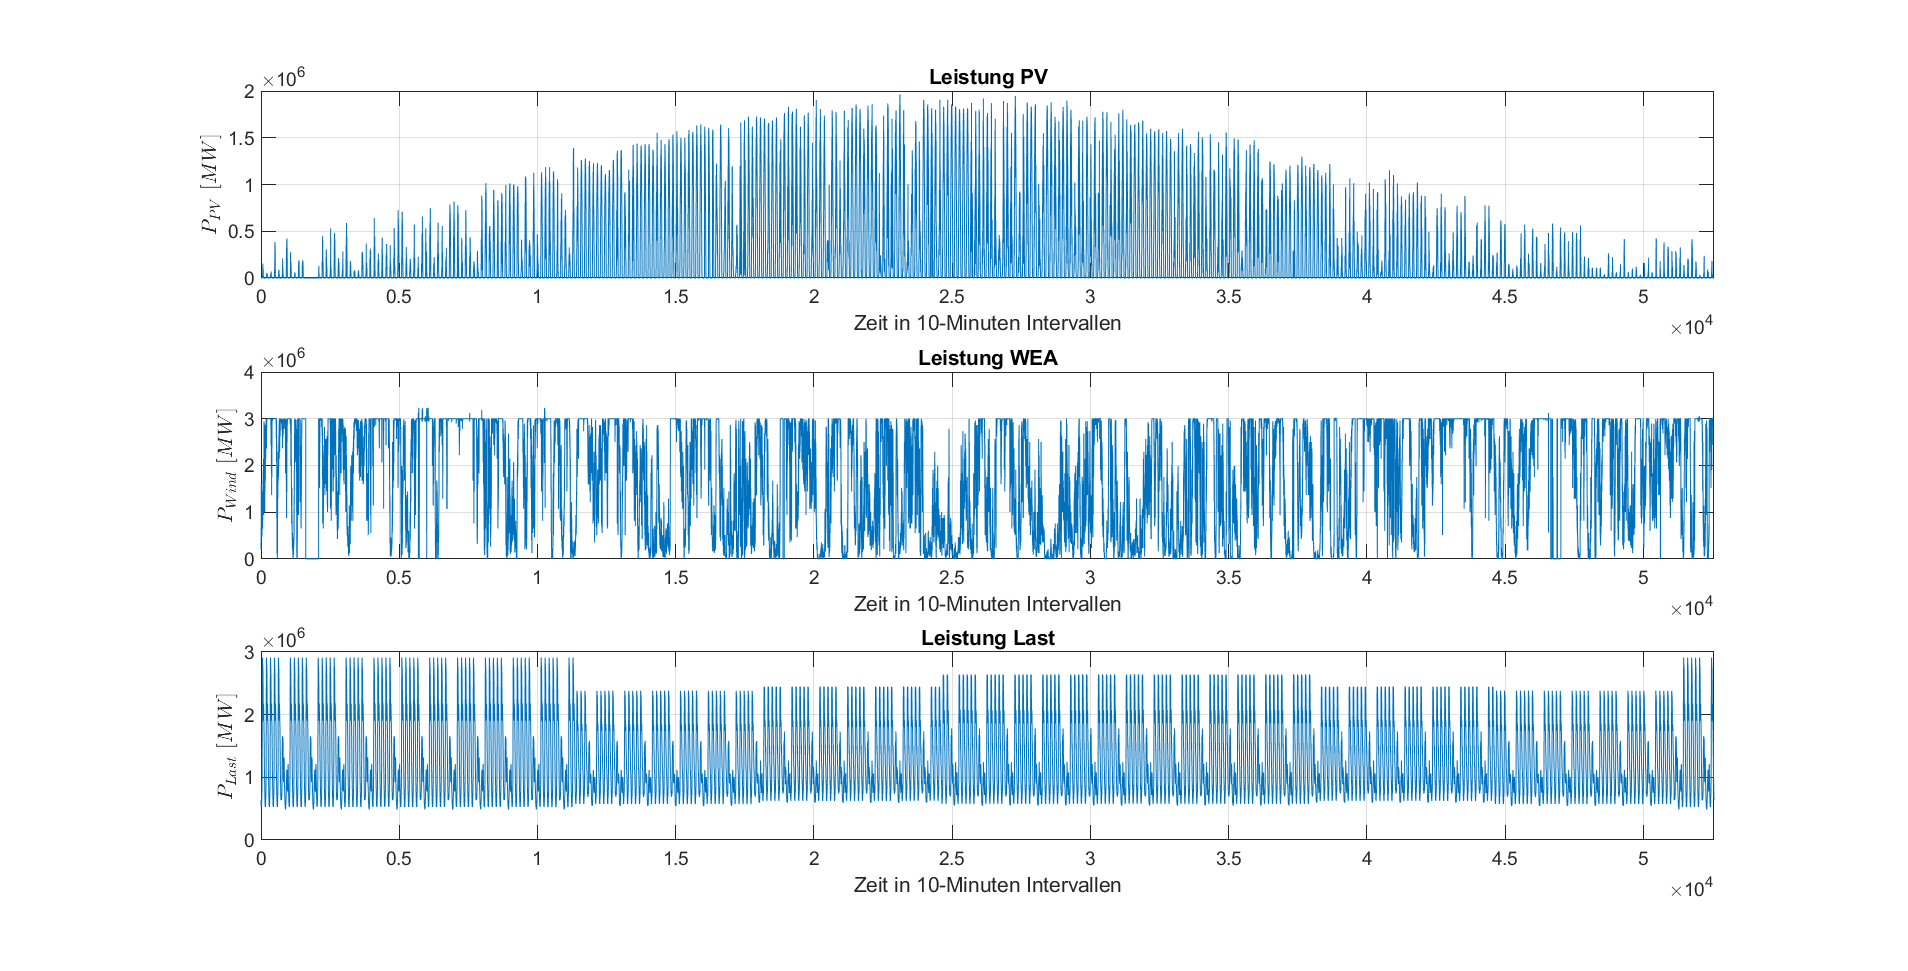
\includegraphics[width=\linewidth]{Abbildungen/HelgolandLeistungOhne.eps}
	\caption{Simulierter Jahresverlauf der Stromproduktion und des Stromverbrauchs}
	\label{fig:helgolandVerlaufOhne}
\end{figure}

Hier ist erneut die starke Abhängigkeit der PV-Produktion von der Jahreszeit erkennbar und es ergibt sich eine jährliche Produktion von 2,3~GWh/a. Zusätzlich steigt der Stromverbrauch im Winter deutlich an. In Summe ist dieser so skaliert, dass er die 11,6 GWh/a aus 2008 erreicht. Die WEA erzeugt durch die vorteilhaften Bedingungen 16,8 GWh/a. Wird nun die Leistungsbilanz gebildet, ergibt sich der Verlauf in \autoref{fig:helgolandBilanzOhne}.

\begin{figure}[H]
	\centering
	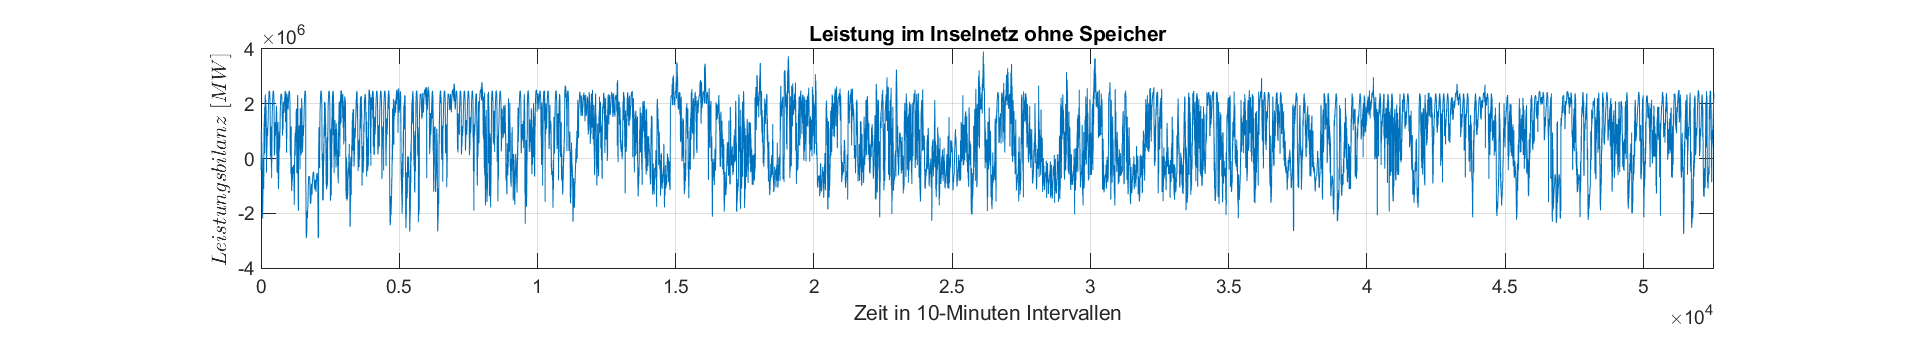
\includegraphics[width=\linewidth]{Abbildungen/HelgolandBilanzOhne.eps}
	\caption{Simulierter Jahresverlauf der Leistungsbilanz im modellierten Inselnetz}
	\label{fig:helgolandBilanzOhne}
\end{figure}

Hier ist klar zu erkennen, dass im schlechtesten Fall keinerlei Produktion vorliegt und ein Speichersystem benötigt wird, welches die komplette Versorgung übernimmt. Daher wird der verwendete Speicher auf eine Lade- und Entladeleistung von 3~MW begrenzt und besitzt eine Kapazität von 300~kWh. Bei erneuter Simulation des Inselnetzes mit Speicher ergebeben sich die Verläufe in \autoref{fig:}

\begin{figure}[H]
	\centering
	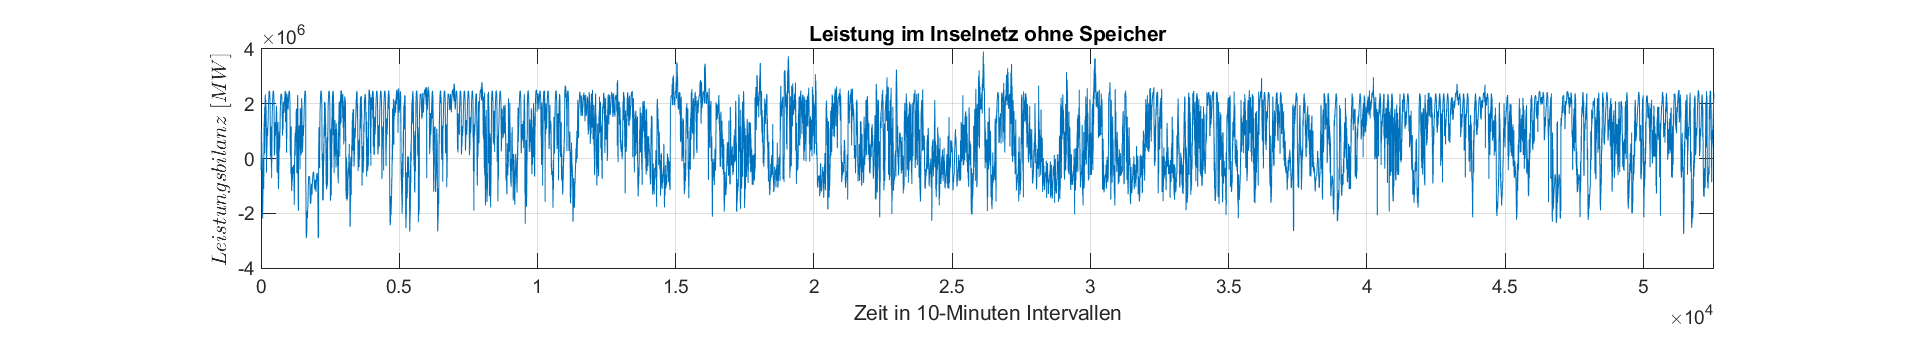
\includegraphics[width=\linewidth]{Abbildungen/HelgolandBilanzOhne.eps}
	\caption{Simulierter Jahresverlauf der Leistungsbilanz im modellierten Inselnetz}
	\label{fig:helgolandBilanzOhne}
\end{figure}

\section{Dreiphasig}

In diesem Abschnitt sollen die Ergebnisse der Simulationen mit dem dreiphasigen Inselnetzmodell diskutiert werden.
Dafür werden zunächst die Parameter und Rahmenbedingungen der Simulation erläutert und anschließend verschiedene 
aufgezeichnete Zeitverläufe präsentiert.
Abschließend soll die Aussagekraft der durchgeführten Simulationen beurteilt und eventuelle Vorschläge 
zur Verbesserung des Modells gemacht werden.

\paragraph{Simulationsparameter}
Um mehrere Simulationen durchzuführen und verschiedene Parameter zu prüfen wurden alle Simulationen auf die Dauer 
des Beispielszenarios aus~\ref{Lade- und Entlade} beschränkt.

Für die Durchführung einer ersten allgemeinen Simulation des Inselnetzes wurden die Verbraucher und die erzeugte
Leistung der Windkraftanlage so ausgelegt, dass sie sich zu Spitzenzeiten in etwa ausgleichen.
Dafür wurde das Lastprofil so gewählt, dass der Verbrauch während der Simulation zwischen 600 kW und 500 kW schwankt.
Die Leistung der Windkraftturbinen schwankt dementsprechend zwischen 0 kW und 600 kW.

Mit dieser Dimensionierung kann einerseits überprüft werden ob der Windkraft-Speicher die Differenz erfolgreich ausgleichen kann
und andererseits muss dieser Speicher so durchgehend positive Leistung bereitstellen und erreicht daher die SOC-Untergrenze.
Ab dieser muss der Speicher sich abschalten, es kommt zu einem Frequenzeinbruch und die FCR wird aktiviert.

\paragraph{Messwerte und Ergebnisse}

\begin{figure}[h!]
	\centering
	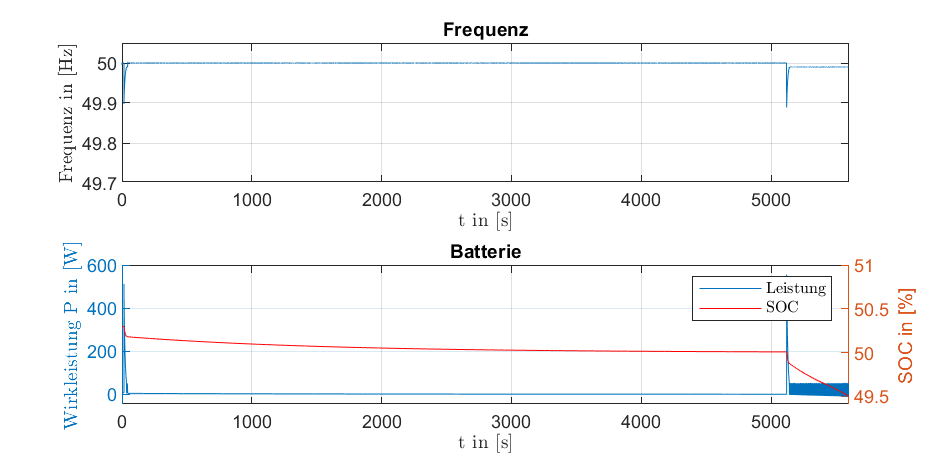
\includegraphics[width=14cm]{Abbildungen/FreqBat2.png}
	\caption{Verlauf der Netzfrequenz und FCR-Batterieleistung}\label{Verlauf1}
\end{figure}

Abbildung~\ref{Verlauf1} zeigt das Verhalten der Netzfrequenz und der Batteriewerte in der grundlegenden Simulation.
Im Verlauf der Frequenz zeigt sich bei 15 s ein Einbruch auf ca 49,9 Hz. 
Zu diesem Zeitpunkt wechselt das Netz in den Inselbetrieb.
Die Batterie stellt sofort 500 kW und damit die halbe Primärrregelleistung zur Verfügung.
Der Generator kann den Frequenzeinbruch abfangen und die Batterieleistung sinkt wieder auf 0 kW.
Während eine konstante Frequenz von 50 Hz gehalten wird, strebt die Batterie einen SOC von 50 \% an.
Da die Abweichung vom Soll-SOC so gering ausfällt zieht die Batterie dabei nur sehr wenig Leistung aus dem Netz.

\begin{figure}[h!]
	\centering
	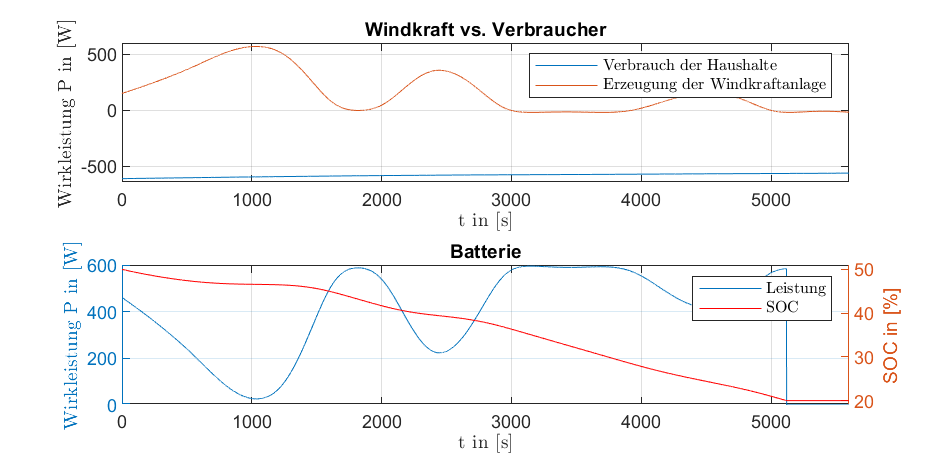
\includegraphics[width=14cm]{Abbildungen/VerbrBat.png}
	\caption{Verlauf der Windkraftleistung, des Lastprofils und der Batterieleistung}\label{Verlauf2}
\end{figure}

Abbildung~\ref{Verlauf2} zeigt den Verlauf der erzeugten Windkraftleistung im Vergleich zur verbrauchten Leistung
und den dazugehörigen Verlauf der Windkraft-Batterieleistung.
Man kann gut erkennen, dass die Batterie die Differenz aus erzeugter und verbrauchter Leistung exakt ausgleichen kann
bis ihr SOC die kritische Grenze von 20 \% erreicht.
In diesem Moment schaltet der Batteriespeicher ab und gibt keine Leistung mehr aus.
In Abbildung~\ref{Verlauf1} bricht zu diesem Zeitpunkt die Frequenz ein.
Diesmal ist der Generator allerdings nicht in der Lage genug Leistung auszugeben um die Frequenz wieder auf ihren
ursprünglichen Wert einzustellen.
Die Batterie zur FCR-Erbringung gibt nun einen konstanten Wert aus und verhindert ein weiteres Absinken der Frequenz aber
es wäre weitere Regelreserve notwendig um wieder eine konstante Netzfrequenz von 50 Hz zu erreichen.
 
\paragraph{Einordnung der Simulation und des Modells}